\section{Classical dynamics towards ($4p$) states}

The ground state properties being established, we will now present the dynamics simulation of the KHe$_N$ system under a $4p\leftarrow 4s$ photo-excitation. 
As already discussed, the $4p$ state is split by interaction with helium and by spin-orbit coupling.
Hence we will present the dynamics following each of the three $\Pi_{1/2}$, $\Pi_{3/2}$ and $\Sigma_{1/2}$ excitations.

\subsection{Quantum versus classical spectra}
\label{sec:4P-spectra}

\begin{figure}[h!]
	\centering
	\begin{minipage}[c]{0.48\linewidth}
		% GNUPLOT: LaTeX picture with Postscript
\begingroup
  \makeatletter
  \providecommand\color[2][]{%
    \GenericError{(gnuplot) \space\space\space\@spaces}{%
      Package color not loaded in conjunction with
      terminal option `colourtext'%
    }{See the gnuplot documentation for explanation.%
    }{Either use 'blacktext' in gnuplot or load the package
      color.sty in LaTeX.}%
    \renewcommand\color[2][]{}%
  }%
  \providecommand\includegraphics[2][]{%
    \GenericError{(gnuplot) \space\space\space\@spaces}{%
      Package graphicx or graphics not loaded%
    }{See the gnuplot documentation for explanation.%
    }{The gnuplot epslatex terminal needs graphicx.sty or graphics.sty.}%
    \renewcommand\includegraphics[2][]{}%
  }%
  \providecommand\rotatebox[2]{#2}%
  \@ifundefined{ifGPcolor}{%
    \newif\ifGPcolor
    \GPcolortrue
  }{}%
  \@ifundefined{ifGPblacktext}{%
    \newif\ifGPblacktext
    \GPblacktextfalse
  }{}%
  % define a \g@addto@macro without @ in the name:
  \let\gplgaddtomacro\g@addto@macro
  % define empty templates for all commands taking text:
  \gdef\gplbacktext{}%
  \gdef\gplfronttext{}%
  \makeatother
  \ifGPblacktext
    % no textcolor at all
    \def\colorrgb#1{}%
    \def\colorgray#1{}%
  \else
    % gray or color?
    \ifGPcolor
      \def\colorrgb#1{\color[rgb]{#1}}%
      \def\colorgray#1{\color[gray]{#1}}%
      \expandafter\def\csname LTw\endcsname{\color{white}}%
      \expandafter\def\csname LTb\endcsname{\color{black}}%
      \expandafter\def\csname LTa\endcsname{\color{black}}%
      \expandafter\def\csname LT0\endcsname{\color[rgb]{1,0,0}}%
      \expandafter\def\csname LT1\endcsname{\color[rgb]{0,1,0}}%
      \expandafter\def\csname LT2\endcsname{\color[rgb]{0,0,1}}%
      \expandafter\def\csname LT3\endcsname{\color[rgb]{1,0,1}}%
      \expandafter\def\csname LT4\endcsname{\color[rgb]{0,1,1}}%
      \expandafter\def\csname LT5\endcsname{\color[rgb]{1,1,0}}%
      \expandafter\def\csname LT6\endcsname{\color[rgb]{0,0,0}}%
      \expandafter\def\csname LT7\endcsname{\color[rgb]{1,0.3,0}}%
      \expandafter\def\csname LT8\endcsname{\color[rgb]{0.5,0.5,0.5}}%
    \else
      % gray
      \def\colorrgb#1{\color{black}}%
      \def\colorgray#1{\color[gray]{#1}}%
      \expandafter\def\csname LTw\endcsname{\color{white}}%
      \expandafter\def\csname LTb\endcsname{\color{black}}%
      \expandafter\def\csname LTa\endcsname{\color{black}}%
      \expandafter\def\csname LT0\endcsname{\color{black}}%
      \expandafter\def\csname LT1\endcsname{\color{black}}%
      \expandafter\def\csname LT2\endcsname{\color{black}}%
      \expandafter\def\csname LT3\endcsname{\color{black}}%
      \expandafter\def\csname LT4\endcsname{\color{black}}%
      \expandafter\def\csname LT5\endcsname{\color{black}}%
      \expandafter\def\csname LT6\endcsname{\color{black}}%
      \expandafter\def\csname LT7\endcsname{\color{black}}%
      \expandafter\def\csname LT8\endcsname{\color{black}}%
    \fi
  \fi
    \setlength{\unitlength}{0.0500bp}%
    \ifx\gptboxheight\undefined%
      \newlength{\gptboxheight}%
      \newlength{\gptboxwidth}%
      \newsavebox{\gptboxtext}%
    \fi%
    \setlength{\fboxrule}{0.5pt}%
    \setlength{\fboxsep}{1pt}%
\begin{picture}(4752.00,2880.00)%
    \gplgaddtomacro\gplbacktext{%
      \csname LTb\endcsname%
      \put(708,432){\makebox(0,0)[r]{\strut{}$0$}}%
      \csname LTb\endcsname%
      \put(708,921){\makebox(0,0)[r]{\strut{}$0.2$}}%
      \csname LTb\endcsname%
      \put(708,1411){\makebox(0,0)[r]{\strut{}$0.4$}}%
      \csname LTb\endcsname%
      \put(708,1900){\makebox(0,0)[r]{\strut{}$0.6$}}%
      \csname LTb\endcsname%
      \put(708,2390){\makebox(0,0)[r]{\strut{}$0.8$}}%
      \csname LTb\endcsname%
      \put(708,2879){\makebox(0,0)[r]{\strut{}$1$}}%
      \csname LTb\endcsname%
      \put(1299,212){\makebox(0,0){\strut{}$13000$}}%
      \csname LTb\endcsname%
      \put(2217,212){\makebox(0,0){\strut{}$13100$}}%
      \csname LTb\endcsname%
      \put(3136,212){\makebox(0,0){\strut{}$13200$}}%
      \csname LTb\endcsname%
      \put(4054,212){\makebox(0,0){\strut{}$13300$}}%
    }%
    \gplgaddtomacro\gplfronttext{%
      \csname LTb\endcsname%
      \put(176,1655){\rotatebox{-270}{\makebox(0,0){\strut{}Intensity (arb. unit)}}}%
      \put(2676,-74){\makebox(0,0){\strut{}Energy (cm$^{-1}$)}}%
      \csname LTb\endcsname%
      \put(3526,2651){\makebox(0,0)[r]{\strut{}$\Sigma_{1/2}$}}%
      \csname LTb\endcsname%
      \put(3526,2431){\makebox(0,0)[r]{\strut{}$\Pi_{3/2}$}}%
      \csname LTb\endcsname%
      \put(3526,2211){\makebox(0,0)[r]{\strut{}$\Pi_{1/2}$}}%
    }%
    \gplbacktext
    \put(0,0){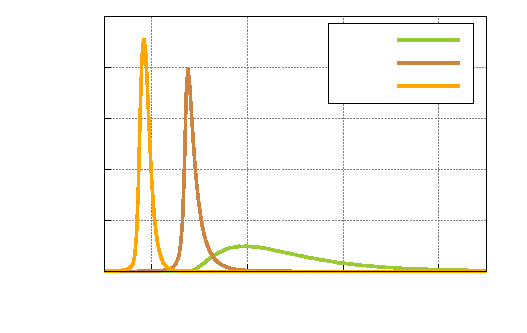
\includegraphics{4P-sp-Q}}%
    \gplfronttext
  \end{picture}%
\endgroup

		\label{fig:4P-sp-Q}
		\vspace{0.2\baselineskip}
		\caption{$4p\rightarrow 4s$ absorption spectra with different state contributions for quantum K}
	\end{minipage}
\hfill
	\begin{minipage}[c]{0.48\linewidth}
		% GNUPLOT: LaTeX picture with Postscript
\begingroup
  \makeatletter
  \providecommand\color[2][]{%
    \GenericError{(gnuplot) \space\space\space\@spaces}{%
      Package color not loaded in conjunction with
      terminal option `colourtext'%
    }{See the gnuplot documentation for explanation.%
    }{Either use 'blacktext' in gnuplot or load the package
      color.sty in LaTeX.}%
    \renewcommand\color[2][]{}%
  }%
  \providecommand\includegraphics[2][]{%
    \GenericError{(gnuplot) \space\space\space\@spaces}{%
      Package graphicx or graphics not loaded%
    }{See the gnuplot documentation for explanation.%
    }{The gnuplot epslatex terminal needs graphicx.sty or graphics.sty.}%
    \renewcommand\includegraphics[2][]{}%
  }%
  \providecommand\rotatebox[2]{#2}%
  \@ifundefined{ifGPcolor}{%
    \newif\ifGPcolor
    \GPcolortrue
  }{}%
  \@ifundefined{ifGPblacktext}{%
    \newif\ifGPblacktext
    \GPblacktextfalse
  }{}%
  % define a \g@addto@macro without @ in the name:
  \let\gplgaddtomacro\g@addto@macro
  % define empty templates for all commands taking text:
  \gdef\gplbacktext{}%
  \gdef\gplfronttext{}%
  \makeatother
  \ifGPblacktext
    % no textcolor at all
    \def\colorrgb#1{}%
    \def\colorgray#1{}%
  \else
    % gray or color?
    \ifGPcolor
      \def\colorrgb#1{\color[rgb]{#1}}%
      \def\colorgray#1{\color[gray]{#1}}%
      \expandafter\def\csname LTw\endcsname{\color{white}}%
      \expandafter\def\csname LTb\endcsname{\color{black}}%
      \expandafter\def\csname LTa\endcsname{\color{black}}%
      \expandafter\def\csname LT0\endcsname{\color[rgb]{1,0,0}}%
      \expandafter\def\csname LT1\endcsname{\color[rgb]{0,1,0}}%
      \expandafter\def\csname LT2\endcsname{\color[rgb]{0,0,1}}%
      \expandafter\def\csname LT3\endcsname{\color[rgb]{1,0,1}}%
      \expandafter\def\csname LT4\endcsname{\color[rgb]{0,1,1}}%
      \expandafter\def\csname LT5\endcsname{\color[rgb]{1,1,0}}%
      \expandafter\def\csname LT6\endcsname{\color[rgb]{0,0,0}}%
      \expandafter\def\csname LT7\endcsname{\color[rgb]{1,0.3,0}}%
      \expandafter\def\csname LT8\endcsname{\color[rgb]{0.5,0.5,0.5}}%
    \else
      % gray
      \def\colorrgb#1{\color{black}}%
      \def\colorgray#1{\color[gray]{#1}}%
      \expandafter\def\csname LTw\endcsname{\color{white}}%
      \expandafter\def\csname LTb\endcsname{\color{black}}%
      \expandafter\def\csname LTa\endcsname{\color{black}}%
      \expandafter\def\csname LT0\endcsname{\color{black}}%
      \expandafter\def\csname LT1\endcsname{\color{black}}%
      \expandafter\def\csname LT2\endcsname{\color{black}}%
      \expandafter\def\csname LT3\endcsname{\color{black}}%
      \expandafter\def\csname LT4\endcsname{\color{black}}%
      \expandafter\def\csname LT5\endcsname{\color{black}}%
      \expandafter\def\csname LT6\endcsname{\color{black}}%
      \expandafter\def\csname LT7\endcsname{\color{black}}%
      \expandafter\def\csname LT8\endcsname{\color{black}}%
    \fi
  \fi
    \setlength{\unitlength}{0.0500bp}%
    \ifx\gptboxheight\undefined%
      \newlength{\gptboxheight}%
      \newlength{\gptboxwidth}%
      \newsavebox{\gptboxtext}%
    \fi%
    \setlength{\fboxrule}{0.5pt}%
    \setlength{\fboxsep}{1pt}%
\begin{picture}(4752.00,2880.00)%
    \gplgaddtomacro\gplbacktext{%
      \csname LTb\endcsname%
      \put(708,432){\makebox(0,0)[r]{\strut{}$0$}}%
      \csname LTb\endcsname%
      \put(708,921){\makebox(0,0)[r]{\strut{}$0.2$}}%
      \csname LTb\endcsname%
      \put(708,1411){\makebox(0,0)[r]{\strut{}$0.4$}}%
      \csname LTb\endcsname%
      \put(708,1900){\makebox(0,0)[r]{\strut{}$0.6$}}%
      \csname LTb\endcsname%
      \put(708,2390){\makebox(0,0)[r]{\strut{}$0.8$}}%
      \csname LTb\endcsname%
      \put(708,2879){\makebox(0,0)[r]{\strut{}$1$}}%
      \csname LTb\endcsname%
      \put(1299,212){\makebox(0,0){\strut{}$13000$}}%
      \csname LTb\endcsname%
      \put(2217,212){\makebox(0,0){\strut{}$13100$}}%
      \csname LTb\endcsname%
      \put(3136,212){\makebox(0,0){\strut{}$13200$}}%
      \csname LTb\endcsname%
      \put(4054,212){\makebox(0,0){\strut{}$13300$}}%
    }%
    \gplgaddtomacro\gplfronttext{%
      \csname LTb\endcsname%
      \put(176,1655){\rotatebox{-270}{\makebox(0,0){\strut{}Intensity (arb. unit)}}}%
      \put(2676,-74){\makebox(0,0){\strut{}Energy (cm$^{-1}$)}}%
      \csname LTb\endcsname%
      \put(3526,2651){\makebox(0,0)[r]{\strut{}Classical}}%
      \csname LTb\endcsname%
      \put(3526,2431){\makebox(0,0)[r]{\strut{}Quantum}}%
      \csname LTb\endcsname%
      \put(3526,2211){\makebox(0,0)[r]{\strut{}Experiment}}%
    }%
    \gplbacktext
    \put(0,0){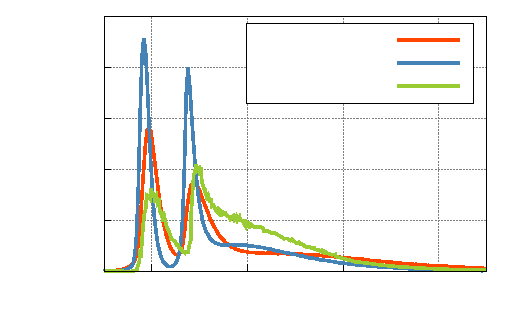
\includegraphics{4P-sp-QC}}%
    \gplfronttext
  \end{picture}%
\endgroup

		\label{fig:4P-sp-QC}
		\vspace{0.2\baselineskip}
		\caption{Comparisons between quantum, classical and experimental spectra \cite{Sti1996}}
	\end{minipage}
\end{figure}

The programs are not yet prepared to describe the quantum motion of K in an anisotropic state.
However, we can still use the quantum ground state density to simulate the spectra with the method described in the  \citanx{sec:ANX-spectra}.
This gives the only opportunity to judge the classical hypothesis for K motion by comparing this spectra to experimental data from \cite{Sti1996}.\\

We clearly see that both the classical and the quantum spectra give a very good agreement.
However,  they fail to describe the relative intensity of the two main peaks and they underestimate the $\Sigma_{1/2}$ component. 
We can conclude that the classical spectrum is really close to the quantum one and to the experimental data, which justifies our hypothesis and validates the potentials used.

\subsection{$\Sigma_{1/2}$ excitation: leaving free potassium}

\begin{figure}[h!]
	\begin{minipage}[c]{0.48\linewidth}
	\hspace{\oldindent} We start our dynamics study with the $\Sigma_{1/2}$ excitation. 
	We observe in \citfig{fig:4P-s12-pos} a fast ejection of the K atom in approximatively 0.2 ps. This behavior could be predicted from \citfig{fig:DIM-4p-pot}, because the averaged interaction is repulsive, however we have to be cautious because this only gives a snapshot of the energy profile at $t=0$ since the droplet is not rigid and can absorb energy from K.\\
	
	 \hspace{\oldindent} We note in \citfig{fig:4P-s12-snap} the global deformation of the droplet during ejection and the creation of density waves in the droplet.\\
	\end{minipage}
\hfill
	\begin{minipage}[c]{0.48\linewidth}
		\fbox{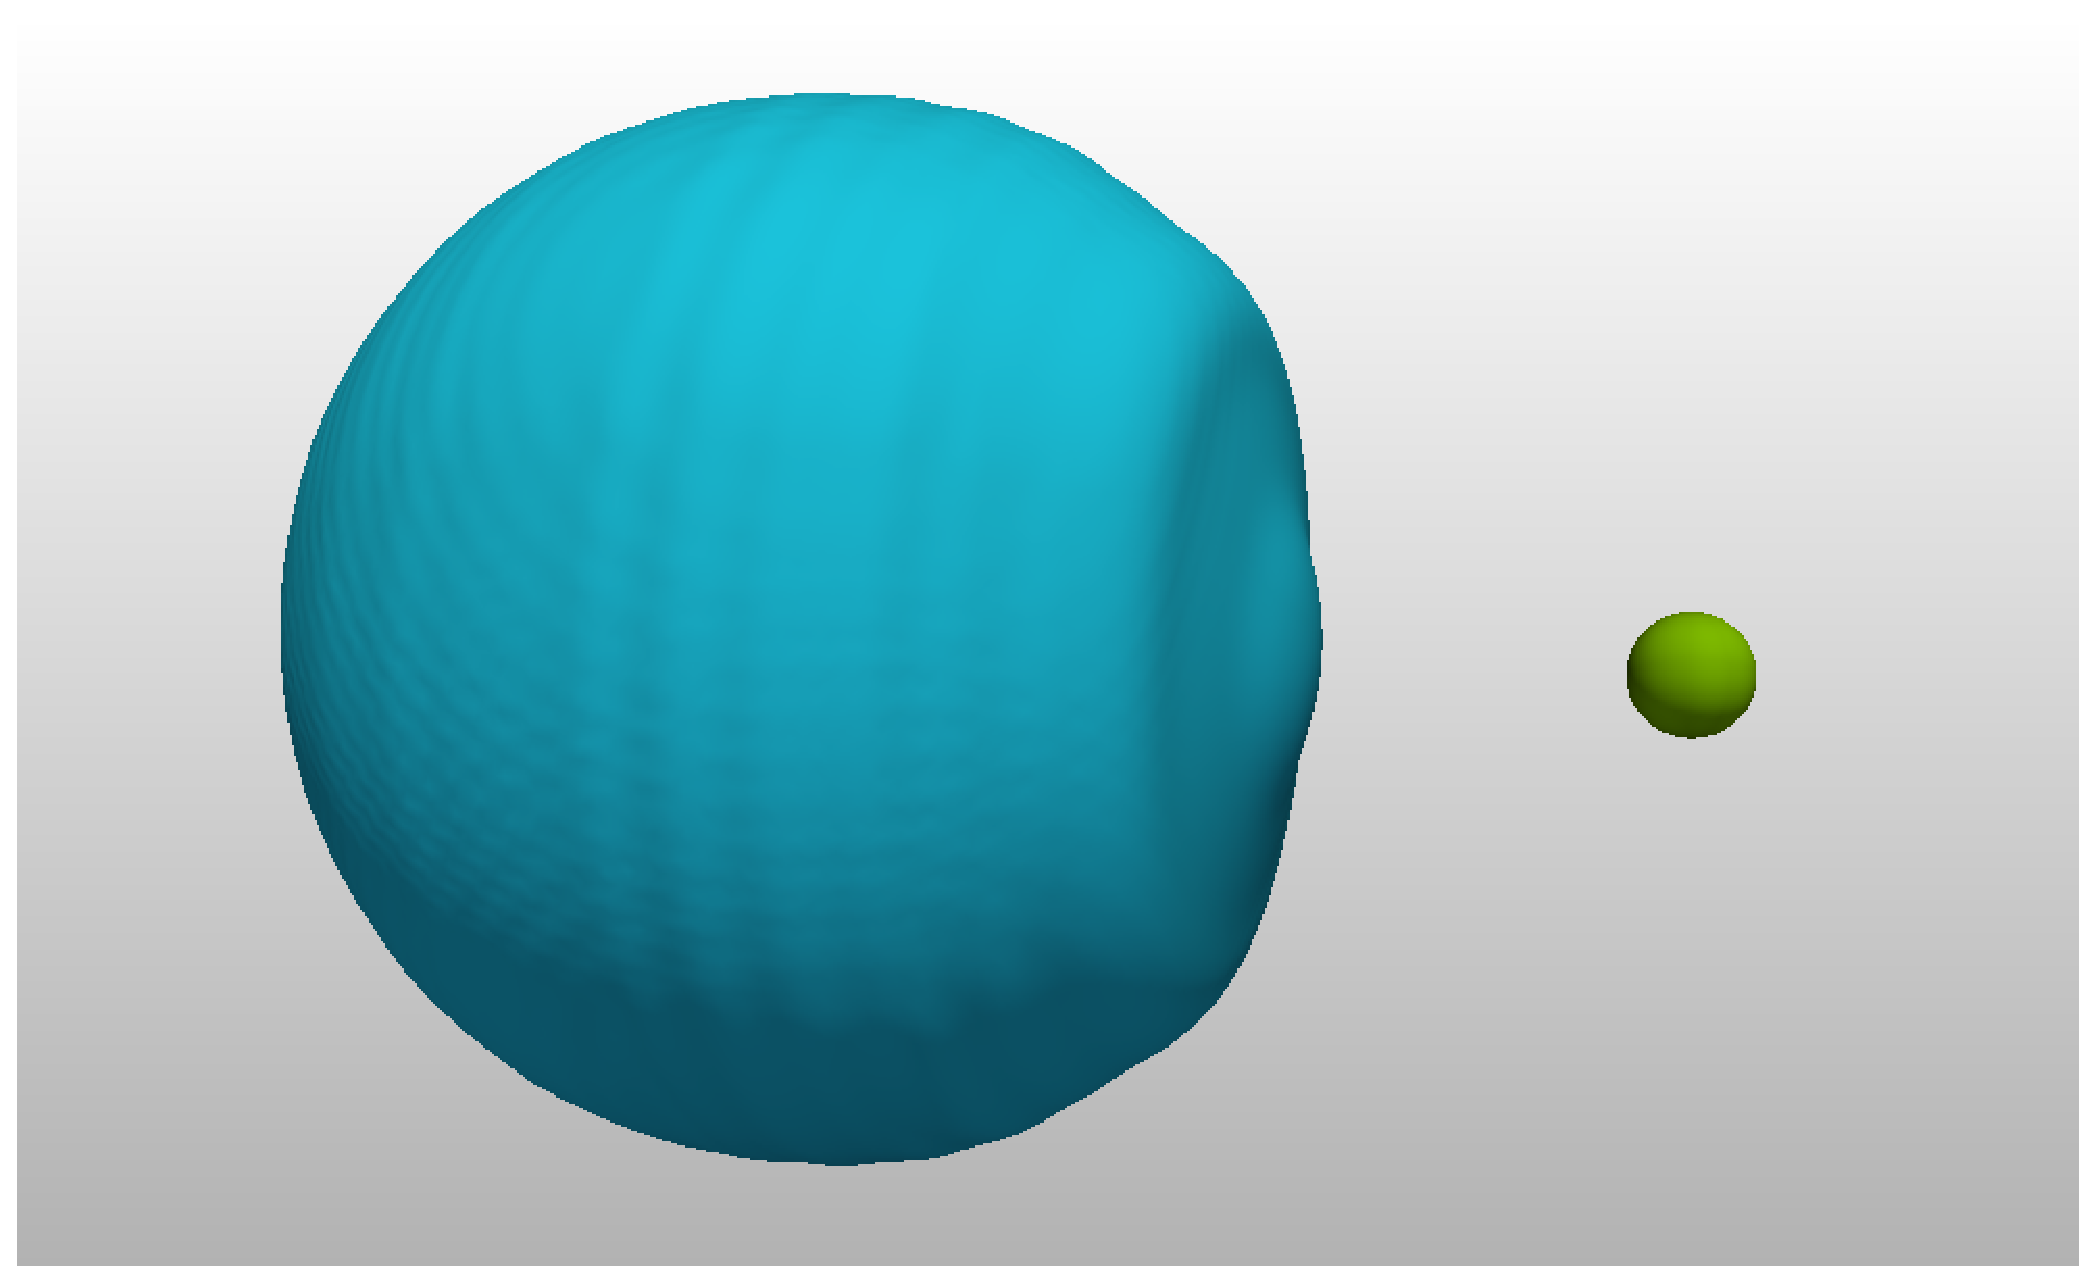
\includegraphics[scale=0.234]{4P-s12-snap}}
		\caption{Snapshot of He$_N$ density and leaving K at $t=8.5$ ps\label{fig:4P-s12-snap}}
	\end{minipage}
\end{figure}

\begin{figure}[h!]
	\centering
	\begin{minipage}[c]{0.48\linewidth}
		% GNUPLOT: LaTeX picture with Postscript
\begingroup
  \makeatletter
  \providecommand\color[2][]{%
    \GenericError{(gnuplot) \space\space\space\@spaces}{%
      Package color not loaded in conjunction with
      terminal option `colourtext'%
    }{See the gnuplot documentation for explanation.%
    }{Either use 'blacktext' in gnuplot or load the package
      color.sty in LaTeX.}%
    \renewcommand\color[2][]{}%
  }%
  \providecommand\includegraphics[2][]{%
    \GenericError{(gnuplot) \space\space\space\@spaces}{%
      Package graphicx or graphics not loaded%
    }{See the gnuplot documentation for explanation.%
    }{The gnuplot epslatex terminal needs graphicx.sty or graphics.sty.}%
    \renewcommand\includegraphics[2][]{}%
  }%
  \providecommand\rotatebox[2]{#2}%
  \@ifundefined{ifGPcolor}{%
    \newif\ifGPcolor
    \GPcolortrue
  }{}%
  \@ifundefined{ifGPblacktext}{%
    \newif\ifGPblacktext
    \GPblacktextfalse
  }{}%
  % define a \g@addto@macro without @ in the name:
  \let\gplgaddtomacro\g@addto@macro
  % define empty templates for all commands taking text:
  \gdef\gplbacktext{}%
  \gdef\gplfronttext{}%
  \makeatother
  \ifGPblacktext
    % no textcolor at all
    \def\colorrgb#1{}%
    \def\colorgray#1{}%
  \else
    % gray or color?
    \ifGPcolor
      \def\colorrgb#1{\color[rgb]{#1}}%
      \def\colorgray#1{\color[gray]{#1}}%
      \expandafter\def\csname LTw\endcsname{\color{white}}%
      \expandafter\def\csname LTb\endcsname{\color{black}}%
      \expandafter\def\csname LTa\endcsname{\color{black}}%
      \expandafter\def\csname LT0\endcsname{\color[rgb]{1,0,0}}%
      \expandafter\def\csname LT1\endcsname{\color[rgb]{0,1,0}}%
      \expandafter\def\csname LT2\endcsname{\color[rgb]{0,0,1}}%
      \expandafter\def\csname LT3\endcsname{\color[rgb]{1,0,1}}%
      \expandafter\def\csname LT4\endcsname{\color[rgb]{0,1,1}}%
      \expandafter\def\csname LT5\endcsname{\color[rgb]{1,1,0}}%
      \expandafter\def\csname LT6\endcsname{\color[rgb]{0,0,0}}%
      \expandafter\def\csname LT7\endcsname{\color[rgb]{1,0.3,0}}%
      \expandafter\def\csname LT8\endcsname{\color[rgb]{0.5,0.5,0.5}}%
    \else
      % gray
      \def\colorrgb#1{\color{black}}%
      \def\colorgray#1{\color[gray]{#1}}%
      \expandafter\def\csname LTw\endcsname{\color{white}}%
      \expandafter\def\csname LTb\endcsname{\color{black}}%
      \expandafter\def\csname LTa\endcsname{\color{black}}%
      \expandafter\def\csname LT0\endcsname{\color{black}}%
      \expandafter\def\csname LT1\endcsname{\color{black}}%
      \expandafter\def\csname LT2\endcsname{\color{black}}%
      \expandafter\def\csname LT3\endcsname{\color{black}}%
      \expandafter\def\csname LT4\endcsname{\color{black}}%
      \expandafter\def\csname LT5\endcsname{\color{black}}%
      \expandafter\def\csname LT6\endcsname{\color{black}}%
      \expandafter\def\csname LT7\endcsname{\color{black}}%
      \expandafter\def\csname LT8\endcsname{\color{black}}%
    \fi
  \fi
    \setlength{\unitlength}{0.0500bp}%
    \ifx\gptboxheight\undefined%
      \newlength{\gptboxheight}%
      \newlength{\gptboxwidth}%
      \newsavebox{\gptboxtext}%
    \fi%
    \setlength{\fboxrule}{0.5pt}%
    \setlength{\fboxsep}{1pt}%
\begin{picture}(4752.00,2880.00)%
    \gplgaddtomacro\gplbacktext{%
      \csname LTb\endcsname%
      \put(708,432){\makebox(0,0)[r]{\strut{}$0$}}%
      \csname LTb\endcsname%
      \put(708,921){\makebox(0,0)[r]{\strut{}$0.2$}}%
      \csname LTb\endcsname%
      \put(708,1411){\makebox(0,0)[r]{\strut{}$0.4$}}%
      \csname LTb\endcsname%
      \put(708,1900){\makebox(0,0)[r]{\strut{}$0.6$}}%
      \csname LTb\endcsname%
      \put(708,2390){\makebox(0,0)[r]{\strut{}$0.8$}}%
      \csname LTb\endcsname%
      \put(708,2879){\makebox(0,0)[r]{\strut{}$1$}}%
      \csname LTb\endcsname%
      \put(840,212){\makebox(0,0){\strut{}$0$}}%
      \csname LTb\endcsname%
      \put(1452,212){\makebox(0,0){\strut{}$2$}}%
      \csname LTb\endcsname%
      \put(2064,212){\makebox(0,0){\strut{}$4$}}%
      \csname LTb\endcsname%
      \put(2677,212){\makebox(0,0){\strut{}$6$}}%
      \csname LTb\endcsname%
      \put(3289,212){\makebox(0,0){\strut{}$8$}}%
      \csname LTb\endcsname%
      \put(3901,212){\makebox(0,0){\strut{}$10$}}%
      \csname LTb\endcsname%
      \put(4513,212){\makebox(0,0){\strut{}$12$}}%
    }%
    \gplgaddtomacro\gplfronttext{%
      \csname LTb\endcsname%
      \put(176,1655){\rotatebox{-270}{\makebox(0,0){\strut{}$|\langle p, s|\lambda\rangle|^2$}}}%
      \put(2676,-74){\makebox(0,0){\strut{}Time (ps)}}%
      \csname LTb\endcsname%
      \put(2837,1766){\makebox(0,0)[r]{\strut{}$\langle p_{1},- |$}}%
      \csname LTb\endcsname%
      \put(2837,1546){\makebox(0,0)[r]{\strut{}$\langle p_{0},+ |$}}%
    }%
    \gplbacktext
    \put(0,0){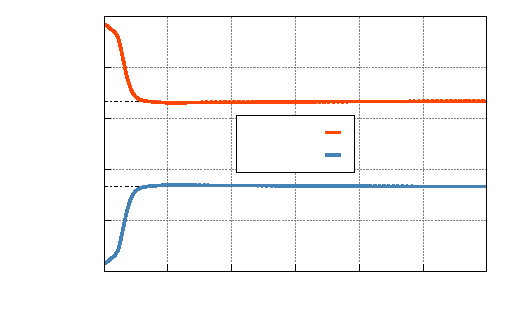
\includegraphics{4P-s12-proj}}%
    \gplfronttext
  \end{picture}%
\endgroup

		\vspace{0.2\baselineskip}
		\caption{Evolution of the electronic state as a function of time\label{fig:4P-s12-proj}}
	\end{minipage}
\hfill
	\begin{minipage}[c]{0.48\linewidth}
		% GNUPLOT: LaTeX picture with Postscript
\begingroup
  \makeatletter
  \providecommand\color[2][]{%
    \GenericError{(gnuplot) \space\space\space\@spaces}{%
      Package color not loaded in conjunction with
      terminal option `colourtext'%
    }{See the gnuplot documentation for explanation.%
    }{Either use 'blacktext' in gnuplot or load the package
      color.sty in LaTeX.}%
    \renewcommand\color[2][]{}%
  }%
  \providecommand\includegraphics[2][]{%
    \GenericError{(gnuplot) \space\space\space\@spaces}{%
      Package graphicx or graphics not loaded%
    }{See the gnuplot documentation for explanation.%
    }{The gnuplot epslatex terminal needs graphicx.sty or graphics.sty.}%
    \renewcommand\includegraphics[2][]{}%
  }%
  \providecommand\rotatebox[2]{#2}%
  \@ifundefined{ifGPcolor}{%
    \newif\ifGPcolor
    \GPcolortrue
  }{}%
  \@ifundefined{ifGPblacktext}{%
    \newif\ifGPblacktext
    \GPblacktextfalse
  }{}%
  % define a \g@addto@macro without @ in the name:
  \let\gplgaddtomacro\g@addto@macro
  % define empty templates for all commands taking text:
  \gdef\gplbacktext{}%
  \gdef\gplfronttext{}%
  \makeatother
  \ifGPblacktext
    % no textcolor at all
    \def\colorrgb#1{}%
    \def\colorgray#1{}%
  \else
    % gray or color?
    \ifGPcolor
      \def\colorrgb#1{\color[rgb]{#1}}%
      \def\colorgray#1{\color[gray]{#1}}%
      \expandafter\def\csname LTw\endcsname{\color{white}}%
      \expandafter\def\csname LTb\endcsname{\color{black}}%
      \expandafter\def\csname LTa\endcsname{\color{black}}%
      \expandafter\def\csname LT0\endcsname{\color[rgb]{1,0,0}}%
      \expandafter\def\csname LT1\endcsname{\color[rgb]{0,1,0}}%
      \expandafter\def\csname LT2\endcsname{\color[rgb]{0,0,1}}%
      \expandafter\def\csname LT3\endcsname{\color[rgb]{1,0,1}}%
      \expandafter\def\csname LT4\endcsname{\color[rgb]{0,1,1}}%
      \expandafter\def\csname LT5\endcsname{\color[rgb]{1,1,0}}%
      \expandafter\def\csname LT6\endcsname{\color[rgb]{0,0,0}}%
      \expandafter\def\csname LT7\endcsname{\color[rgb]{1,0.3,0}}%
      \expandafter\def\csname LT8\endcsname{\color[rgb]{0.5,0.5,0.5}}%
    \else
      % gray
      \def\colorrgb#1{\color{black}}%
      \def\colorgray#1{\color[gray]{#1}}%
      \expandafter\def\csname LTw\endcsname{\color{white}}%
      \expandafter\def\csname LTb\endcsname{\color{black}}%
      \expandafter\def\csname LTa\endcsname{\color{black}}%
      \expandafter\def\csname LT0\endcsname{\color{black}}%
      \expandafter\def\csname LT1\endcsname{\color{black}}%
      \expandafter\def\csname LT2\endcsname{\color{black}}%
      \expandafter\def\csname LT3\endcsname{\color{black}}%
      \expandafter\def\csname LT4\endcsname{\color{black}}%
      \expandafter\def\csname LT5\endcsname{\color{black}}%
      \expandafter\def\csname LT6\endcsname{\color{black}}%
      \expandafter\def\csname LT7\endcsname{\color{black}}%
      \expandafter\def\csname LT8\endcsname{\color{black}}%
    \fi
  \fi
    \setlength{\unitlength}{0.0500bp}%
    \ifx\gptboxheight\undefined%
      \newlength{\gptboxheight}%
      \newlength{\gptboxwidth}%
      \newsavebox{\gptboxtext}%
    \fi%
    \setlength{\fboxrule}{0.5pt}%
    \setlength{\fboxsep}{1pt}%
\begin{picture}(4752.00,2880.00)%
    \gplgaddtomacro\gplbacktext{%
      \csname LTb\endcsname%
      \put(946,432){\makebox(0,0)[r]{\strut{}$26.1$}}%
      \csname LTb\endcsname%
      \put(946,921){\makebox(0,0)[r]{\strut{}$26.4$}}%
      \csname LTb\endcsname%
      \put(946,1411){\makebox(0,0)[r]{\strut{}$26.7$}}%
      \csname LTb\endcsname%
      \put(946,1900){\makebox(0,0)[r]{\strut{}$27$}}%
      \csname LTb\endcsname%
      \put(946,2390){\makebox(0,0)[r]{\strut{}$27.3$}}%
      \csname LTb\endcsname%
      \put(946,2879){\makebox(0,0)[r]{\strut{}$27.6$}}%
      \csname LTb\endcsname%
      \put(1078,212){\makebox(0,0){\strut{}$0$}}%
      \csname LTb\endcsname%
      \put(1651,212){\makebox(0,0){\strut{}$0.2$}}%
      \csname LTb\endcsname%
      \put(2223,212){\makebox(0,0){\strut{}$0.4$}}%
      \csname LTb\endcsname%
      \put(2796,212){\makebox(0,0){\strut{}$0.6$}}%
      \csname LTb\endcsname%
      \put(3368,212){\makebox(0,0){\strut{}$0.8$}}%
      \csname LTb\endcsname%
      \put(3941,212){\makebox(0,0){\strut{}$1$}}%
      \csname LTb\endcsname%
      \put(4513,212){\makebox(0,0){\strut{}$1.2$}}%
    }%
    \gplgaddtomacro\gplfronttext{%
      \csname LTb\endcsname%
      \put(176,1655){\rotatebox{-270}{\makebox(0,0){\strut{}K relative position (\AA)}}}%
      \put(2795,-74){\makebox(0,0){\strut{}Time (ps)}}%
    }%
    \gplbacktext
    \put(0,0){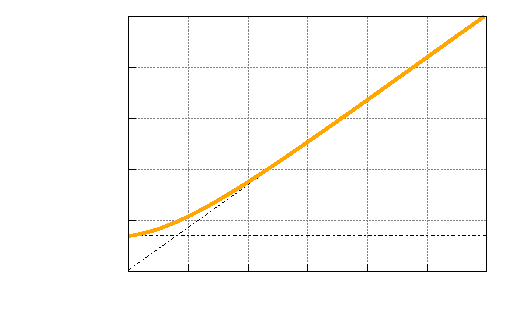
\includegraphics{4P-s12-pos}}%
    \gplfronttext
  \end{picture}%
\endgroup

		\vspace{0.2\baselineskip}
		\caption{Distance between K and He$_N$ centers of mass as a function of time\label{fig:4P-s12-pos}}
	\end{minipage}
\end{figure}

The study of the evolution of the internal electronic state will be important in following discussions, this is why we start discussing it for $\Sigma_{1/2}$ as a simple case. 
We saw in \citsec{sec:DIM-dia} that $\Omega$ is the only true good quantum number.
Here we have $\Omega=1/2$\footnote{We only discuss the positive case but the reasoning is the same for $\Omega=-1/2$ since they are degenerate}.
This can be checked in \citfig{fig:4P-s12-proj} since it is a linear combination of $\ket{p_1,-}$ and $\ket{p_0,+}$.
In addition we have seen that $\Lambda$ should be a good quantum number in the excitation region (\citsec{sec:DIM-dia}).
For the  $\Sigma_{1/2}$  state $\Lambda\approx 0$, which is why $\ket{p_0,+}$ is dominant at $t=0$.
Finally we can see that once K is far from droplet, its internal state becomes an eigenvector of $\vb{J}^2$ with eigenvalue $J=3/2$.
This is also expected because $J$ is a good quantum number in this region and the  $\Sigma_{1/2}$ state connects asymptotically to $J=3/2$  (\citsec{sec:DIM-4p})
\begin{align}
\ket{\lambda} \underset{t\rightarrow \infty}{\longrightarrow} \ket{J=3/2,\Omega=1/2} = \sqrt{\frac{1}{3}} \ket{p_1,-} + \sqrt{\frac{2}{3}} \ket{p_0,+}
\end{align}

\subsection{$\Pi_{1/2}$ excitation: complexity arises}

\subsubsection{Bouncing potassium}

\begin{figure}[h!]
	\centering
	\begin{minipage}[c]{0.48\linewidth}
		% GNUPLOT: LaTeX picture with Postscript
\begingroup
  \makeatletter
  \providecommand\color[2][]{%
    \GenericError{(gnuplot) \space\space\space\@spaces}{%
      Package color not loaded in conjunction with
      terminal option `colourtext'%
    }{See the gnuplot documentation for explanation.%
    }{Either use 'blacktext' in gnuplot or load the package
      color.sty in LaTeX.}%
    \renewcommand\color[2][]{}%
  }%
  \providecommand\includegraphics[2][]{%
    \GenericError{(gnuplot) \space\space\space\@spaces}{%
      Package graphicx or graphics not loaded%
    }{See the gnuplot documentation for explanation.%
    }{The gnuplot epslatex terminal needs graphicx.sty or graphics.sty.}%
    \renewcommand\includegraphics[2][]{}%
  }%
  \providecommand\rotatebox[2]{#2}%
  \@ifundefined{ifGPcolor}{%
    \newif\ifGPcolor
    \GPcolortrue
  }{}%
  \@ifundefined{ifGPblacktext}{%
    \newif\ifGPblacktext
    \GPblacktextfalse
  }{}%
  % define a \g@addto@macro without @ in the name:
  \let\gplgaddtomacro\g@addto@macro
  % define empty templates for all commands taking text:
  \gdef\gplbacktext{}%
  \gdef\gplfronttext{}%
  \makeatother
  \ifGPblacktext
    % no textcolor at all
    \def\colorrgb#1{}%
    \def\colorgray#1{}%
  \else
    % gray or color?
    \ifGPcolor
      \def\colorrgb#1{\color[rgb]{#1}}%
      \def\colorgray#1{\color[gray]{#1}}%
      \expandafter\def\csname LTw\endcsname{\color{white}}%
      \expandafter\def\csname LTb\endcsname{\color{black}}%
      \expandafter\def\csname LTa\endcsname{\color{black}}%
      \expandafter\def\csname LT0\endcsname{\color[rgb]{1,0,0}}%
      \expandafter\def\csname LT1\endcsname{\color[rgb]{0,1,0}}%
      \expandafter\def\csname LT2\endcsname{\color[rgb]{0,0,1}}%
      \expandafter\def\csname LT3\endcsname{\color[rgb]{1,0,1}}%
      \expandafter\def\csname LT4\endcsname{\color[rgb]{0,1,1}}%
      \expandafter\def\csname LT5\endcsname{\color[rgb]{1,1,0}}%
      \expandafter\def\csname LT6\endcsname{\color[rgb]{0,0,0}}%
      \expandafter\def\csname LT7\endcsname{\color[rgb]{1,0.3,0}}%
      \expandafter\def\csname LT8\endcsname{\color[rgb]{0.5,0.5,0.5}}%
    \else
      % gray
      \def\colorrgb#1{\color{black}}%
      \def\colorgray#1{\color[gray]{#1}}%
      \expandafter\def\csname LTw\endcsname{\color{white}}%
      \expandafter\def\csname LTb\endcsname{\color{black}}%
      \expandafter\def\csname LTa\endcsname{\color{black}}%
      \expandafter\def\csname LT0\endcsname{\color{black}}%
      \expandafter\def\csname LT1\endcsname{\color{black}}%
      \expandafter\def\csname LT2\endcsname{\color{black}}%
      \expandafter\def\csname LT3\endcsname{\color{black}}%
      \expandafter\def\csname LT4\endcsname{\color{black}}%
      \expandafter\def\csname LT5\endcsname{\color{black}}%
      \expandafter\def\csname LT6\endcsname{\color{black}}%
      \expandafter\def\csname LT7\endcsname{\color{black}}%
      \expandafter\def\csname LT8\endcsname{\color{black}}%
    \fi
  \fi
    \setlength{\unitlength}{0.0500bp}%
    \ifx\gptboxheight\undefined%
      \newlength{\gptboxheight}%
      \newlength{\gptboxwidth}%
      \newsavebox{\gptboxtext}%
    \fi%
    \setlength{\fboxrule}{0.5pt}%
    \setlength{\fboxsep}{1pt}%
\begin{picture}(4752.00,2880.00)%
    \gplgaddtomacro\gplbacktext{%
      \csname LTb\endcsname%
      \put(682,432){\makebox(0,0)[r]{\strut{}$26$}}%
      \csname LTb\endcsname%
      \put(682,782){\makebox(0,0)[r]{\strut{}$28$}}%
      \csname LTb\endcsname%
      \put(682,1131){\makebox(0,0)[r]{\strut{}$30$}}%
      \csname LTb\endcsname%
      \put(682,1481){\makebox(0,0)[r]{\strut{}$32$}}%
      \csname LTb\endcsname%
      \put(682,1830){\makebox(0,0)[r]{\strut{}$34$}}%
      \csname LTb\endcsname%
      \put(682,2180){\makebox(0,0)[r]{\strut{}$36$}}%
      \csname LTb\endcsname%
      \put(682,2529){\makebox(0,0)[r]{\strut{}$38$}}%
      \csname LTb\endcsname%
      \put(682,2879){\makebox(0,0)[r]{\strut{}$40$}}%
      \csname LTb\endcsname%
      \put(814,212){\makebox(0,0){\strut{}$0$}}%
      \csname LTb\endcsname%
      \put(1431,212){\makebox(0,0){\strut{}$40$}}%
      \csname LTb\endcsname%
      \put(2047,212){\makebox(0,0){\strut{}$80$}}%
      \csname LTb\endcsname%
      \put(2664,212){\makebox(0,0){\strut{}$120$}}%
      \csname LTb\endcsname%
      \put(3280,212){\makebox(0,0){\strut{}$160$}}%
      \csname LTb\endcsname%
      \put(3897,212){\makebox(0,0){\strut{}$200$}}%
      \csname LTb\endcsname%
      \put(4513,212){\makebox(0,0){\strut{}$240$}}%
    }%
    \gplgaddtomacro\gplfronttext{%
      \csname LTb\endcsname%
      \put(176,1655){\rotatebox{-270}{\makebox(0,0){\strut{}K relative position (\AA)}}}%
      \put(2663,-74){\makebox(0,0){\strut{}Time (ps)}}%
    }%
    \gplbacktext
    \put(0,0){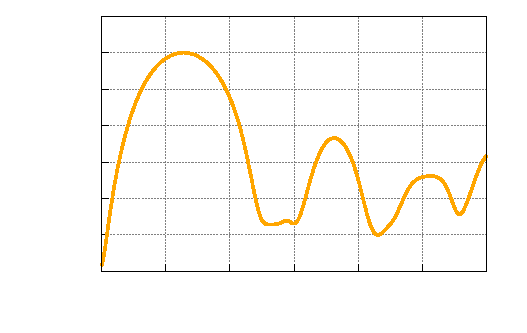
\includegraphics{4P-p12-pos}}%
    \gplfronttext
  \end{picture}%
\endgroup

		\vspace{0.2\baselineskip}
		\caption{Distance between K and He$_N$ centers of mass as a function of time\label{fig:4P-p12-n-pos}}
	\end{minipage}
\hfill
	\begin{minipage}[c]{0.48\linewidth}
		\fbox{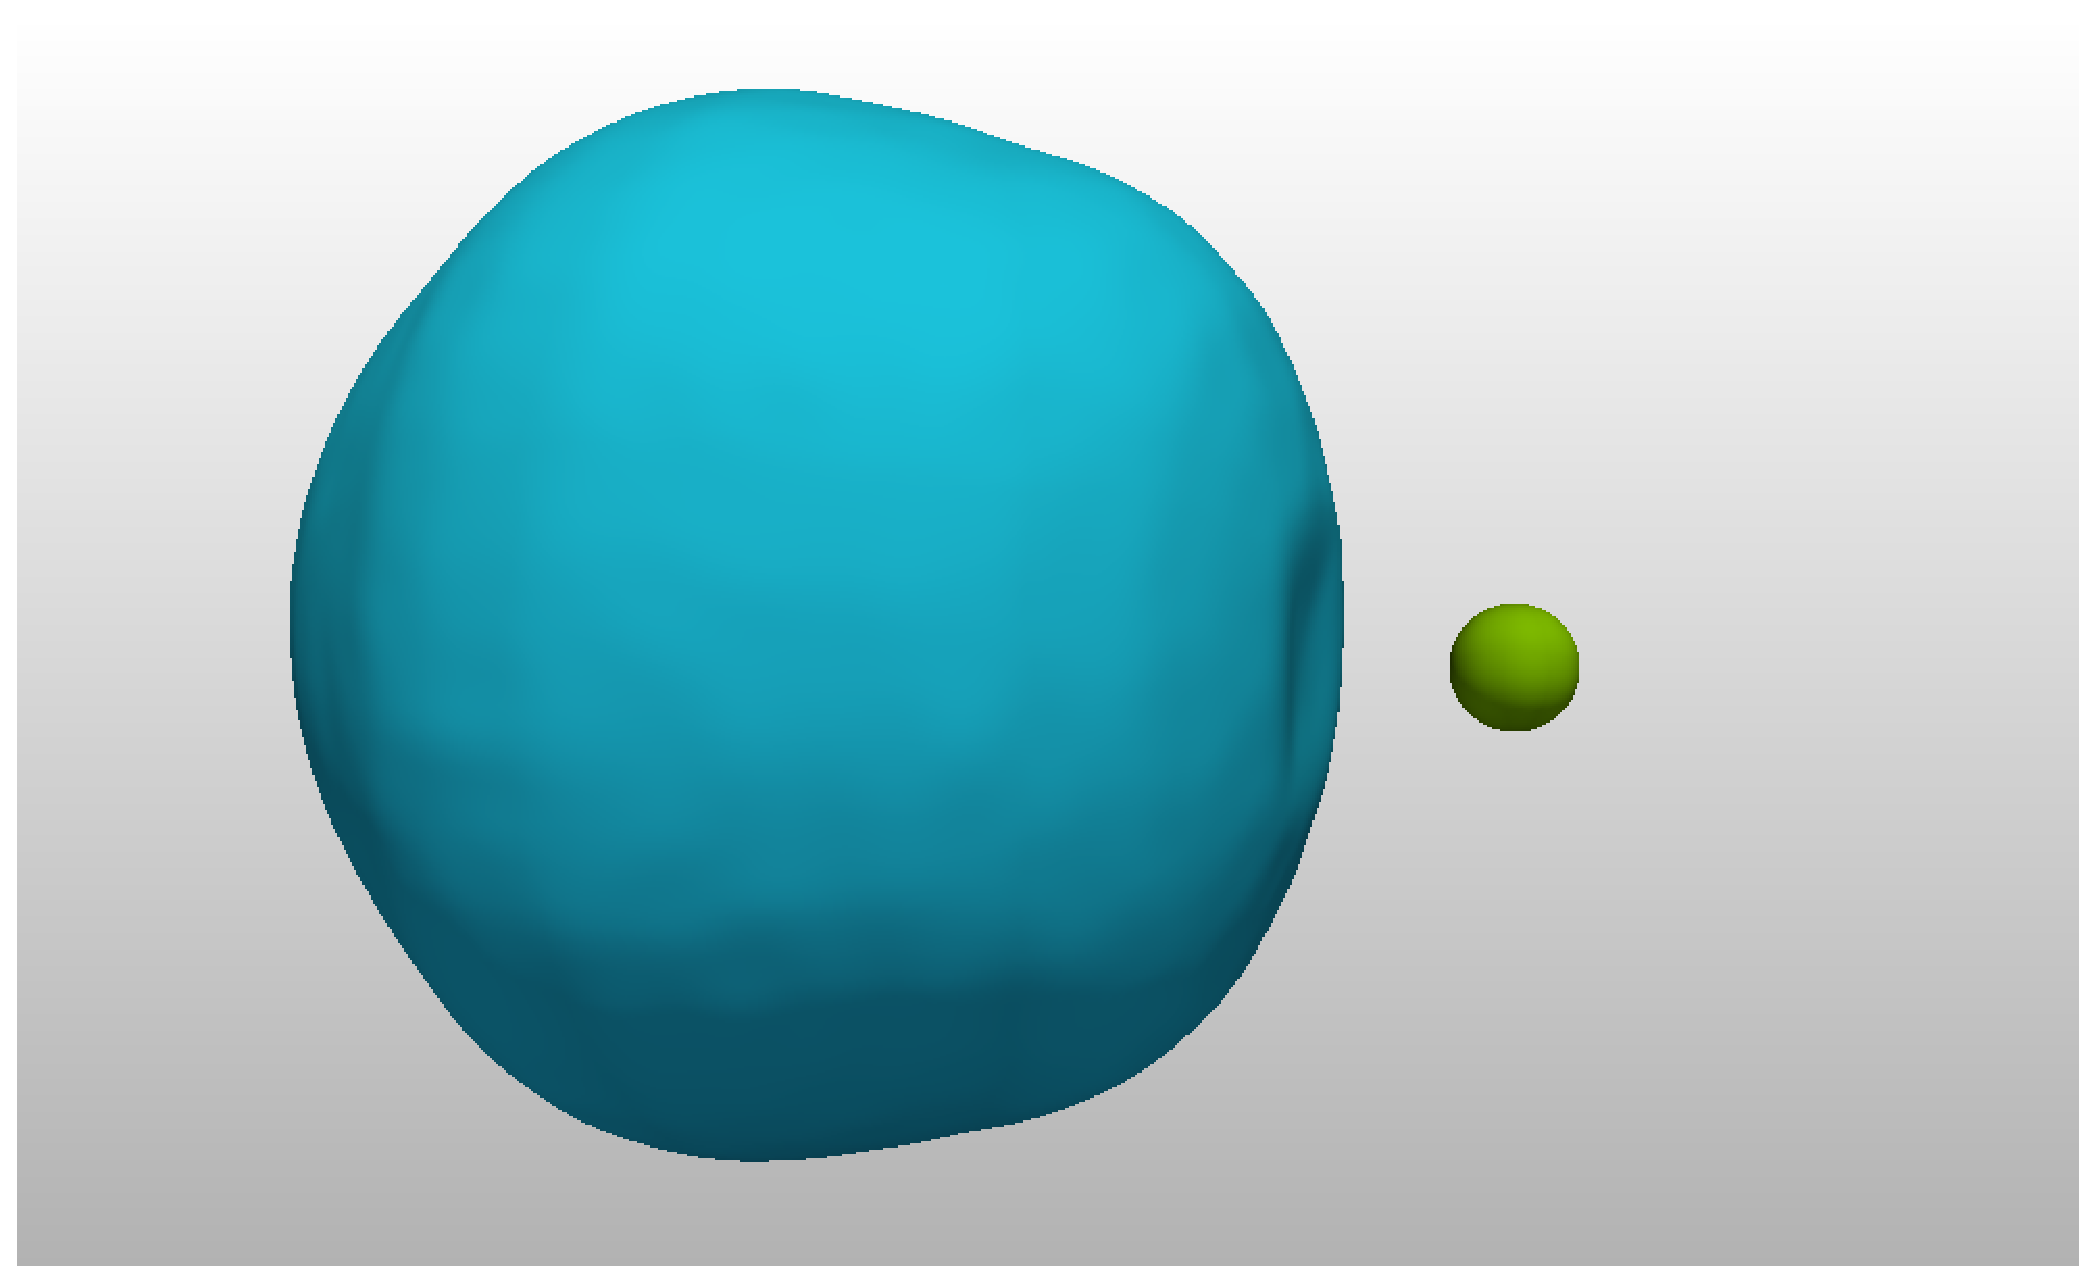
\includegraphics[scale=0.234]{4P-p12-n-snap}}
		\caption{Snapshot of He$_N$ density and bouncing K at $t=182$ ps \label{fig:4P-p12-n-snap}}
	\end{minipage}
\end{figure}

\begin{figure}[h!]
\centering
	\begin{minipage}[c]{0.48\linewidth}
		% GNUPLOT: LaTeX picture with Postscript
\begingroup
  \makeatletter
  \providecommand\color[2][]{%
    \GenericError{(gnuplot) \space\space\space\@spaces}{%
      Package color not loaded in conjunction with
      terminal option `colourtext'%
    }{See the gnuplot documentation for explanation.%
    }{Either use 'blacktext' in gnuplot or load the package
      color.sty in LaTeX.}%
    \renewcommand\color[2][]{}%
  }%
  \providecommand\includegraphics[2][]{%
    \GenericError{(gnuplot) \space\space\space\@spaces}{%
      Package graphicx or graphics not loaded%
    }{See the gnuplot documentation for explanation.%
    }{The gnuplot epslatex terminal needs graphicx.sty or graphics.sty.}%
    \renewcommand\includegraphics[2][]{}%
  }%
  \providecommand\rotatebox[2]{#2}%
  \@ifundefined{ifGPcolor}{%
    \newif\ifGPcolor
    \GPcolortrue
  }{}%
  \@ifundefined{ifGPblacktext}{%
    \newif\ifGPblacktext
    \GPblacktextfalse
  }{}%
  % define a \g@addto@macro without @ in the name:
  \let\gplgaddtomacro\g@addto@macro
  % define empty templates for all commands taking text:
  \gdef\gplbacktext{}%
  \gdef\gplfronttext{}%
  \makeatother
  \ifGPblacktext
    % no textcolor at all
    \def\colorrgb#1{}%
    \def\colorgray#1{}%
  \else
    % gray or color?
    \ifGPcolor
      \def\colorrgb#1{\color[rgb]{#1}}%
      \def\colorgray#1{\color[gray]{#1}}%
      \expandafter\def\csname LTw\endcsname{\color{white}}%
      \expandafter\def\csname LTb\endcsname{\color{black}}%
      \expandafter\def\csname LTa\endcsname{\color{black}}%
      \expandafter\def\csname LT0\endcsname{\color[rgb]{1,0,0}}%
      \expandafter\def\csname LT1\endcsname{\color[rgb]{0,1,0}}%
      \expandafter\def\csname LT2\endcsname{\color[rgb]{0,0,1}}%
      \expandafter\def\csname LT3\endcsname{\color[rgb]{1,0,1}}%
      \expandafter\def\csname LT4\endcsname{\color[rgb]{0,1,1}}%
      \expandafter\def\csname LT5\endcsname{\color[rgb]{1,1,0}}%
      \expandafter\def\csname LT6\endcsname{\color[rgb]{0,0,0}}%
      \expandafter\def\csname LT7\endcsname{\color[rgb]{1,0.3,0}}%
      \expandafter\def\csname LT8\endcsname{\color[rgb]{0.5,0.5,0.5}}%
    \else
      % gray
      \def\colorrgb#1{\color{black}}%
      \def\colorgray#1{\color[gray]{#1}}%
      \expandafter\def\csname LTw\endcsname{\color{white}}%
      \expandafter\def\csname LTb\endcsname{\color{black}}%
      \expandafter\def\csname LTa\endcsname{\color{black}}%
      \expandafter\def\csname LT0\endcsname{\color{black}}%
      \expandafter\def\csname LT1\endcsname{\color{black}}%
      \expandafter\def\csname LT2\endcsname{\color{black}}%
      \expandafter\def\csname LT3\endcsname{\color{black}}%
      \expandafter\def\csname LT4\endcsname{\color{black}}%
      \expandafter\def\csname LT5\endcsname{\color{black}}%
      \expandafter\def\csname LT6\endcsname{\color{black}}%
      \expandafter\def\csname LT7\endcsname{\color{black}}%
      \expandafter\def\csname LT8\endcsname{\color{black}}%
    \fi
  \fi
    \setlength{\unitlength}{0.0500bp}%
    \ifx\gptboxheight\undefined%
      \newlength{\gptboxheight}%
      \newlength{\gptboxwidth}%
      \newsavebox{\gptboxtext}%
    \fi%
    \setlength{\fboxrule}{0.5pt}%
    \setlength{\fboxsep}{1pt}%
\begin{picture}(4752.00,2880.00)%
    \gplgaddtomacro\gplbacktext{%
      \csname LTb\endcsname%
      \put(708,432){\makebox(0,0)[r]{\strut{}$0$}}%
      \csname LTb\endcsname%
      \put(708,921){\makebox(0,0)[r]{\strut{}$0.2$}}%
      \csname LTb\endcsname%
      \put(708,1411){\makebox(0,0)[r]{\strut{}$0.4$}}%
      \csname LTb\endcsname%
      \put(708,1900){\makebox(0,0)[r]{\strut{}$0.6$}}%
      \csname LTb\endcsname%
      \put(708,2390){\makebox(0,0)[r]{\strut{}$0.8$}}%
      \csname LTb\endcsname%
      \put(708,2879){\makebox(0,0)[r]{\strut{}$1$}}%
      \csname LTb\endcsname%
      \put(840,212){\makebox(0,0){\strut{}$0$}}%
      \csname LTb\endcsname%
      \put(1452,212){\makebox(0,0){\strut{}$40$}}%
      \csname LTb\endcsname%
      \put(2064,212){\makebox(0,0){\strut{}$80$}}%
      \csname LTb\endcsname%
      \put(2677,212){\makebox(0,0){\strut{}$120$}}%
      \csname LTb\endcsname%
      \put(3289,212){\makebox(0,0){\strut{}$160$}}%
      \csname LTb\endcsname%
      \put(3901,212){\makebox(0,0){\strut{}$200$}}%
      \csname LTb\endcsname%
      \put(4513,212){\makebox(0,0){\strut{}$240$}}%
    }%
    \gplgaddtomacro\gplfronttext{%
      \csname LTb\endcsname%
      \put(176,1655){\rotatebox{-270}{\makebox(0,0){\strut{}$|\langle p, s|\lambda\rangle|^2$}}}%
      \put(2676,-74){\makebox(0,0){\strut{}Time (ps)}}%
      \csname LTb\endcsname%
      \put(2837,1766){\makebox(0,0)[r]{\strut{}$\langle p_{1},- |$}}%
      \csname LTb\endcsname%
      \put(2837,1546){\makebox(0,0)[r]{\strut{}$\langle p_{0},+ |$}}%
    }%
    \gplbacktext
    \put(0,0){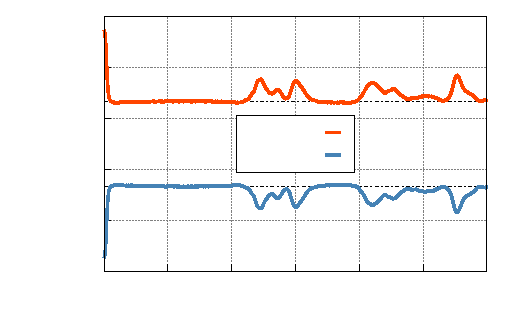
\includegraphics{4P-p12-n-proj}}%
    \gplfronttext
  \end{picture}%
\endgroup

		\vspace{0.2\baselineskip}
		\caption{Evolution of the electronic state as a function of time\label{fig:4P-p12-n-proj}}
	\end{minipage}
\hfill
	\begin{minipage}[c]{0.48\linewidth}
		% GNUPLOT: LaTeX picture with Postscript
\begingroup
  \makeatletter
  \providecommand\color[2][]{%
    \GenericError{(gnuplot) \space\space\space\@spaces}{%
      Package color not loaded in conjunction with
      terminal option `colourtext'%
    }{See the gnuplot documentation for explanation.%
    }{Either use 'blacktext' in gnuplot or load the package
      color.sty in LaTeX.}%
    \renewcommand\color[2][]{}%
  }%
  \providecommand\includegraphics[2][]{%
    \GenericError{(gnuplot) \space\space\space\@spaces}{%
      Package graphicx or graphics not loaded%
    }{See the gnuplot documentation for explanation.%
    }{The gnuplot epslatex terminal needs graphicx.sty or graphics.sty.}%
    \renewcommand\includegraphics[2][]{}%
  }%
  \providecommand\rotatebox[2]{#2}%
  \@ifundefined{ifGPcolor}{%
    \newif\ifGPcolor
    \GPcolortrue
  }{}%
  \@ifundefined{ifGPblacktext}{%
    \newif\ifGPblacktext
    \GPblacktextfalse
  }{}%
  % define a \g@addto@macro without @ in the name:
  \let\gplgaddtomacro\g@addto@macro
  % define empty templates for all commands taking text:
  \gdef\gplbacktext{}%
  \gdef\gplfronttext{}%
  \makeatother
  \ifGPblacktext
    % no textcolor at all
    \def\colorrgb#1{}%
    \def\colorgray#1{}%
  \else
    % gray or color?
    \ifGPcolor
      \def\colorrgb#1{\color[rgb]{#1}}%
      \def\colorgray#1{\color[gray]{#1}}%
      \expandafter\def\csname LTw\endcsname{\color{white}}%
      \expandafter\def\csname LTb\endcsname{\color{black}}%
      \expandafter\def\csname LTa\endcsname{\color{black}}%
      \expandafter\def\csname LT0\endcsname{\color[rgb]{1,0,0}}%
      \expandafter\def\csname LT1\endcsname{\color[rgb]{0,1,0}}%
      \expandafter\def\csname LT2\endcsname{\color[rgb]{0,0,1}}%
      \expandafter\def\csname LT3\endcsname{\color[rgb]{1,0,1}}%
      \expandafter\def\csname LT4\endcsname{\color[rgb]{0,1,1}}%
      \expandafter\def\csname LT5\endcsname{\color[rgb]{1,1,0}}%
      \expandafter\def\csname LT6\endcsname{\color[rgb]{0,0,0}}%
      \expandafter\def\csname LT7\endcsname{\color[rgb]{1,0.3,0}}%
      \expandafter\def\csname LT8\endcsname{\color[rgb]{0.5,0.5,0.5}}%
    \else
      % gray
      \def\colorrgb#1{\color{black}}%
      \def\colorgray#1{\color[gray]{#1}}%
      \expandafter\def\csname LTw\endcsname{\color{white}}%
      \expandafter\def\csname LTb\endcsname{\color{black}}%
      \expandafter\def\csname LTa\endcsname{\color{black}}%
      \expandafter\def\csname LT0\endcsname{\color{black}}%
      \expandafter\def\csname LT1\endcsname{\color{black}}%
      \expandafter\def\csname LT2\endcsname{\color{black}}%
      \expandafter\def\csname LT3\endcsname{\color{black}}%
      \expandafter\def\csname LT4\endcsname{\color{black}}%
      \expandafter\def\csname LT5\endcsname{\color{black}}%
      \expandafter\def\csname LT6\endcsname{\color{black}}%
      \expandafter\def\csname LT7\endcsname{\color{black}}%
      \expandafter\def\csname LT8\endcsname{\color{black}}%
    \fi
  \fi
    \setlength{\unitlength}{0.0500bp}%
    \ifx\gptboxheight\undefined%
      \newlength{\gptboxheight}%
      \newlength{\gptboxwidth}%
      \newsavebox{\gptboxtext}%
    \fi%
    \setlength{\fboxrule}{0.5pt}%
    \setlength{\fboxsep}{1pt}%
\begin{picture}(4752.00,2880.00)%
    \gplgaddtomacro\gplbacktext{%
      \csname LTb\endcsname%
      \put(814,432){\makebox(0,0)[r]{\strut{}$-60$}}%
      \csname LTb\endcsname%
      \put(814,782){\makebox(0,0)[r]{\strut{}$-55$}}%
      \csname LTb\endcsname%
      \put(814,1131){\makebox(0,0)[r]{\strut{}$-50$}}%
      \csname LTb\endcsname%
      \put(814,1481){\makebox(0,0)[r]{\strut{}$-45$}}%
      \csname LTb\endcsname%
      \put(814,1830){\makebox(0,0)[r]{\strut{}$-40$}}%
      \csname LTb\endcsname%
      \put(814,2180){\makebox(0,0)[r]{\strut{}$-35$}}%
      \csname LTb\endcsname%
      \put(814,2529){\makebox(0,0)[r]{\strut{}$-30$}}%
      \csname LTb\endcsname%
      \put(814,2879){\makebox(0,0)[r]{\strut{}$-25$}}%
      \csname LTb\endcsname%
      \put(946,212){\makebox(0,0){\strut{}$0$}}%
      \csname LTb\endcsname%
      \put(1541,212){\makebox(0,0){\strut{}$1$}}%
      \csname LTb\endcsname%
      \put(2135,212){\makebox(0,0){\strut{}$2$}}%
      \csname LTb\endcsname%
      \put(2730,212){\makebox(0,0){\strut{}$3$}}%
      \csname LTb\endcsname%
      \put(3324,212){\makebox(0,0){\strut{}$4$}}%
      \csname LTb\endcsname%
      \put(3919,212){\makebox(0,0){\strut{}$5$}}%
      \csname LTb\endcsname%
      \put(4513,212){\makebox(0,0){\strut{}$6$}}%
    }%
    \gplgaddtomacro\gplfronttext{%
      \csname LTb\endcsname%
      \put(176,1655){\rotatebox{-270}{\makebox(0,0){\strut{}Impurity energy (K)}}}%
      \put(2729,-74){\makebox(0,0){\strut{}Time (ps)}}%
    }%
    \gplbacktext
    \put(0,0){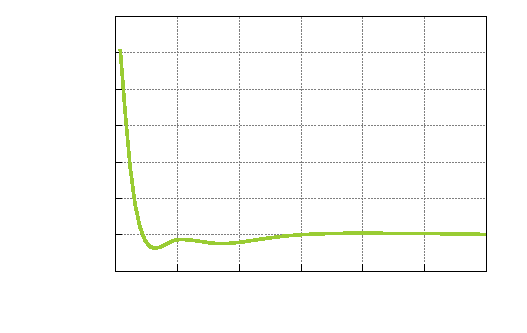
\includegraphics{4P-p12-energy}}%
    \gplfronttext
  \end{picture}%
\endgroup

		\vspace{0.2\baselineskip}
		\caption{Total potassium energy as a function of time\label{fig:4P-p12-n-energy}}
	\end{minipage}
\end{figure}
	
After excitation to the $\Pi_{1/2}$ state the potassium does not leave the droplet as can be seen in \citfig{fig:4P-p12-n-pos}.
Moreover the 3D snapshot \citfig{fig:4P-p12-n-snap} shows no exciplex formation. 
This behavior can look surprising at first  because  the pair potential is repulsive and the averaged potential shows that K has enough potential energy at $t=0$ to dissociate (cf \citfig{fig:DIM-4p-pot}). 
One can actually easily understand what is going on by plotting the total impurity energy as a function of time.
As shown in \citfig{fig:4P-p12-n-energy}, K is giving a lot of energy to the droplet: up to 25 K. 
On the other hand the $\Pi_{1/2}$ pair potential has a tiny well about +4.0 \AA{} away from the initial position, which creates both a long range attraction and a barrier when the particle is coming back. 
These two phenomena explain why we have a bouncing-bound K.
In particular we see that the bouncing occurs at around +2.5 \AA{}, which is consistent with the previous explanation. 
One can also understand why there is no exciplex formation: the deep well in the pair potential is not accessible due to the tiny barrier.\\

The electronic state evolution for $\Pi_{1/2}$ excitation is presented in \citfig{fig:4P-p12-n-proj}.
The situation is similar to that of $\Sigma_{1/2}$ excitation because $\Omega=1/2$, but here $\Lambda \approx 1$ and $J\approx 1/2$ so that $\ket{p_1,-}$ is dominant at small distance and we find $\ket{J=1/2,\Omega=1/2}$ at large distances.
In particular we note that when K is bouncing we are in an intermediate case.

\subsubsection{Displacing the excitation position}

The previous discussion showed that the tiny barrier close to the excitation region plays an important role. 
It is therefore interesting to see what happens when the initial position of K is slightly shifted.
This could occur either due to thermal excitation or to quantum delocalization.
One can use diabatic potentials and ground state K wave function (see \citfig{fig:4S-potentials}) to determine the order of magnitude of a reasonable shift.
It appears that both thermal (0.4~K) and quantum (half of the maximum of the wave function) fluctuations give a possible $\pm$0.5 \AA{} shift for the excitation position.
%
\begin{figure}[h!]
\centering
	\begin{minipage}[c]{0.48\linewidth}
		% GNUPLOT: LaTeX picture with Postscript
\begingroup
  \makeatletter
  \providecommand\color[2][]{%
    \GenericError{(gnuplot) \space\space\space\@spaces}{%
      Package color not loaded in conjunction with
      terminal option `colourtext'%
    }{See the gnuplot documentation for explanation.%
    }{Either use 'blacktext' in gnuplot or load the package
      color.sty in LaTeX.}%
    \renewcommand\color[2][]{}%
  }%
  \providecommand\includegraphics[2][]{%
    \GenericError{(gnuplot) \space\space\space\@spaces}{%
      Package graphicx or graphics not loaded%
    }{See the gnuplot documentation for explanation.%
    }{The gnuplot epslatex terminal needs graphicx.sty or graphics.sty.}%
    \renewcommand\includegraphics[2][]{}%
  }%
  \providecommand\rotatebox[2]{#2}%
  \@ifundefined{ifGPcolor}{%
    \newif\ifGPcolor
    \GPcolortrue
  }{}%
  \@ifundefined{ifGPblacktext}{%
    \newif\ifGPblacktext
    \GPblacktextfalse
  }{}%
  % define a \g@addto@macro without @ in the name:
  \let\gplgaddtomacro\g@addto@macro
  % define empty templates for all commands taking text:
  \gdef\gplbacktext{}%
  \gdef\gplfronttext{}%
  \makeatother
  \ifGPblacktext
    % no textcolor at all
    \def\colorrgb#1{}%
    \def\colorgray#1{}%
  \else
    % gray or color?
    \ifGPcolor
      \def\colorrgb#1{\color[rgb]{#1}}%
      \def\colorgray#1{\color[gray]{#1}}%
      \expandafter\def\csname LTw\endcsname{\color{white}}%
      \expandafter\def\csname LTb\endcsname{\color{black}}%
      \expandafter\def\csname LTa\endcsname{\color{black}}%
      \expandafter\def\csname LT0\endcsname{\color[rgb]{1,0,0}}%
      \expandafter\def\csname LT1\endcsname{\color[rgb]{0,1,0}}%
      \expandafter\def\csname LT2\endcsname{\color[rgb]{0,0,1}}%
      \expandafter\def\csname LT3\endcsname{\color[rgb]{1,0,1}}%
      \expandafter\def\csname LT4\endcsname{\color[rgb]{0,1,1}}%
      \expandafter\def\csname LT5\endcsname{\color[rgb]{1,1,0}}%
      \expandafter\def\csname LT6\endcsname{\color[rgb]{0,0,0}}%
      \expandafter\def\csname LT7\endcsname{\color[rgb]{1,0.3,0}}%
      \expandafter\def\csname LT8\endcsname{\color[rgb]{0.5,0.5,0.5}}%
    \else
      % gray
      \def\colorrgb#1{\color{black}}%
      \def\colorgray#1{\color[gray]{#1}}%
      \expandafter\def\csname LTw\endcsname{\color{white}}%
      \expandafter\def\csname LTb\endcsname{\color{black}}%
      \expandafter\def\csname LTa\endcsname{\color{black}}%
      \expandafter\def\csname LT0\endcsname{\color{black}}%
      \expandafter\def\csname LT1\endcsname{\color{black}}%
      \expandafter\def\csname LT2\endcsname{\color{black}}%
      \expandafter\def\csname LT3\endcsname{\color{black}}%
      \expandafter\def\csname LT4\endcsname{\color{black}}%
      \expandafter\def\csname LT5\endcsname{\color{black}}%
      \expandafter\def\csname LT6\endcsname{\color{black}}%
      \expandafter\def\csname LT7\endcsname{\color{black}}%
      \expandafter\def\csname LT8\endcsname{\color{black}}%
    \fi
  \fi
    \setlength{\unitlength}{0.0500bp}%
    \ifx\gptboxheight\undefined%
      \newlength{\gptboxheight}%
      \newlength{\gptboxwidth}%
      \newsavebox{\gptboxtext}%
    \fi%
    \setlength{\fboxrule}{0.5pt}%
    \setlength{\fboxsep}{1pt}%
\begin{picture}(4752.00,2880.00)%
    \gplgaddtomacro\gplbacktext{%
      \csname LTb\endcsname%
      \put(814,432){\makebox(0,0)[r]{\strut{}$0$}}%
      \csname LTb\endcsname%
      \put(814,921){\makebox(0,0)[r]{\strut{}$0.2$}}%
      \csname LTb\endcsname%
      \put(814,1411){\makebox(0,0)[r]{\strut{}$0.4$}}%
      \csname LTb\endcsname%
      \put(814,1900){\makebox(0,0)[r]{\strut{}$0.6$}}%
      \csname LTb\endcsname%
      \put(814,2390){\makebox(0,0)[r]{\strut{}$0.8$}}%
      \csname LTb\endcsname%
      \put(814,2879){\makebox(0,0)[r]{\strut{}$1$}}%
      \csname LTb\endcsname%
      \put(946,212){\makebox(0,0){\strut{}$0$}}%
      \csname LTb\endcsname%
      \put(1838,212){\makebox(0,0){\strut{}$4$}}%
      \csname LTb\endcsname%
      \put(2730,212){\makebox(0,0){\strut{}$8$}}%
      \csname LTb\endcsname%
      \put(3621,212){\makebox(0,0){\strut{}$12$}}%
      \csname LTb\endcsname%
      \put(4513,212){\makebox(0,0){\strut{}$16$}}%
    }%
    \gplgaddtomacro\gplfronttext{%
      \csname LTb\endcsname%
      \put(176,1655){\rotatebox{-270}{\makebox(0,0){\strut{}Intensity (arb. unit)}}}%
      \put(2729,-74){\makebox(0,0){\strut{}Energy (cm$^{-1}$)}}%
      \csname LTb\endcsname%
      \put(2209,2096){\makebox(0,0)[r]{\strut{}$\langle p_{+1},-|$}}%
      \csname LTb\endcsname%
      \put(2209,1876){\makebox(0,0)[r]{\strut{}$\langle p_{-1},-|$}}%
      \csname LTb\endcsname%
      \put(2209,1656){\makebox(0,0)[r]{\strut{}$\langle p_{0},+|$}}%
      \csname LTb\endcsname%
      \put(2209,1436){\makebox(0,0)[r]{\strut{}$\langle p_{x},-|$}}%
      \csname LTb\endcsname%
      \put(2209,1216){\makebox(0,0)[r]{\strut{}$\langle p_{y},-|$}}%
    }%
    \gplbacktext
    \put(0,0){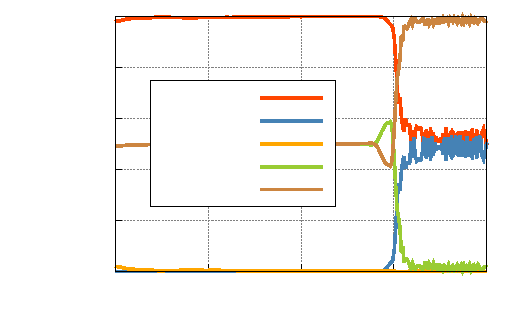
\includegraphics{4P-p12-d-proj}}%
    \gplfronttext
  \end{picture}%
\endgroup

		\vspace{0.2\baselineskip}
		\caption{Evolution of the electronic state as a function of time\label{fig:4P-p12-d-proj}}
	\end{minipage}
\hfill
	\begin{minipage}[c]{0.48\linewidth}
		% GNUPLOT: LaTeX picture with Postscript
\begingroup
  \makeatletter
  \providecommand\color[2][]{%
    \GenericError{(gnuplot) \space\space\space\@spaces}{%
      Package color not loaded in conjunction with
      terminal option `colourtext'%
    }{See the gnuplot documentation for explanation.%
    }{Either use 'blacktext' in gnuplot or load the package
      color.sty in LaTeX.}%
    \renewcommand\color[2][]{}%
  }%
  \providecommand\includegraphics[2][]{%
    \GenericError{(gnuplot) \space\space\space\@spaces}{%
      Package graphicx or graphics not loaded%
    }{See the gnuplot documentation for explanation.%
    }{The gnuplot epslatex terminal needs graphicx.sty or graphics.sty.}%
    \renewcommand\includegraphics[2][]{}%
  }%
  \providecommand\rotatebox[2]{#2}%
  \@ifundefined{ifGPcolor}{%
    \newif\ifGPcolor
    \GPcolortrue
  }{}%
  \@ifundefined{ifGPblacktext}{%
    \newif\ifGPblacktext
    \GPblacktextfalse
  }{}%
  % define a \g@addto@macro without @ in the name:
  \let\gplgaddtomacro\g@addto@macro
  % define empty templates for all commands taking text:
  \gdef\gplbacktext{}%
  \gdef\gplfronttext{}%
  \makeatother
  \ifGPblacktext
    % no textcolor at all
    \def\colorrgb#1{}%
    \def\colorgray#1{}%
  \else
    % gray or color?
    \ifGPcolor
      \def\colorrgb#1{\color[rgb]{#1}}%
      \def\colorgray#1{\color[gray]{#1}}%
      \expandafter\def\csname LTw\endcsname{\color{white}}%
      \expandafter\def\csname LTb\endcsname{\color{black}}%
      \expandafter\def\csname LTa\endcsname{\color{black}}%
      \expandafter\def\csname LT0\endcsname{\color[rgb]{1,0,0}}%
      \expandafter\def\csname LT1\endcsname{\color[rgb]{0,1,0}}%
      \expandafter\def\csname LT2\endcsname{\color[rgb]{0,0,1}}%
      \expandafter\def\csname LT3\endcsname{\color[rgb]{1,0,1}}%
      \expandafter\def\csname LT4\endcsname{\color[rgb]{0,1,1}}%
      \expandafter\def\csname LT5\endcsname{\color[rgb]{1,1,0}}%
      \expandafter\def\csname LT6\endcsname{\color[rgb]{0,0,0}}%
      \expandafter\def\csname LT7\endcsname{\color[rgb]{1,0.3,0}}%
      \expandafter\def\csname LT8\endcsname{\color[rgb]{0.5,0.5,0.5}}%
    \else
      % gray
      \def\colorrgb#1{\color{black}}%
      \def\colorgray#1{\color[gray]{#1}}%
      \expandafter\def\csname LTw\endcsname{\color{white}}%
      \expandafter\def\csname LTb\endcsname{\color{black}}%
      \expandafter\def\csname LTa\endcsname{\color{black}}%
      \expandafter\def\csname LT0\endcsname{\color{black}}%
      \expandafter\def\csname LT1\endcsname{\color{black}}%
      \expandafter\def\csname LT2\endcsname{\color{black}}%
      \expandafter\def\csname LT3\endcsname{\color{black}}%
      \expandafter\def\csname LT4\endcsname{\color{black}}%
      \expandafter\def\csname LT5\endcsname{\color{black}}%
      \expandafter\def\csname LT6\endcsname{\color{black}}%
      \expandafter\def\csname LT7\endcsname{\color{black}}%
      \expandafter\def\csname LT8\endcsname{\color{black}}%
    \fi
  \fi
    \setlength{\unitlength}{0.0500bp}%
    \ifx\gptboxheight\undefined%
      \newlength{\gptboxheight}%
      \newlength{\gptboxwidth}%
      \newsavebox{\gptboxtext}%
    \fi%
    \setlength{\fboxrule}{0.5pt}%
    \setlength{\fboxsep}{1pt}%
\begin{picture}(4752.00,2880.00)%
    \gplgaddtomacro\gplbacktext{%
      \csname LTb\endcsname%
      \put(682,432){\makebox(0,0)[r]{\strut{}$25$}}%
      \csname LTb\endcsname%
      \put(682,840){\makebox(0,0)[r]{\strut{}$26$}}%
      \csname LTb\endcsname%
      \put(682,1248){\makebox(0,0)[r]{\strut{}$27$}}%
      \csname LTb\endcsname%
      \put(682,1656){\makebox(0,0)[r]{\strut{}$28$}}%
      \csname LTb\endcsname%
      \put(682,2063){\makebox(0,0)[r]{\strut{}$29$}}%
      \csname LTb\endcsname%
      \put(682,2471){\makebox(0,0)[r]{\strut{}$30$}}%
      \csname LTb\endcsname%
      \put(682,2879){\makebox(0,0)[r]{\strut{}$31$}}%
      \csname LTb\endcsname%
      \put(814,212){\makebox(0,0){\strut{}$0$}}%
      \csname LTb\endcsname%
      \put(1431,212){\makebox(0,0){\strut{}$10$}}%
      \csname LTb\endcsname%
      \put(2047,212){\makebox(0,0){\strut{}$20$}}%
      \csname LTb\endcsname%
      \put(2664,212){\makebox(0,0){\strut{}$30$}}%
      \csname LTb\endcsname%
      \put(3280,212){\makebox(0,0){\strut{}$40$}}%
      \csname LTb\endcsname%
      \put(3897,212){\makebox(0,0){\strut{}$50$}}%
      \csname LTb\endcsname%
      \put(4513,212){\makebox(0,0){\strut{}$60$}}%
    }%
    \gplgaddtomacro\gplfronttext{%
      \csname LTb\endcsname%
      \put(176,1655){\rotatebox{-270}{\makebox(0,0){\strut{}K relative position (\AA)}}}%
      \put(2663,-74){\makebox(0,0){\strut{}Time (ps)}}%
    }%
    \gplbacktext
    \put(0,0){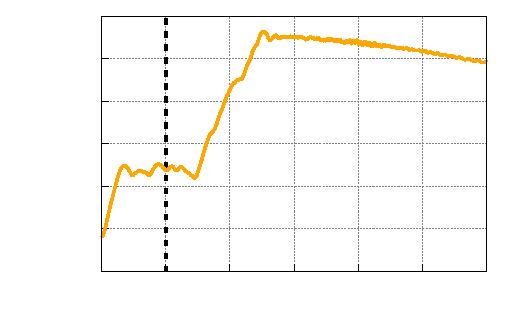
\includegraphics{4P-p12-d-pos}}%
    \gplfronttext
  \end{picture}%
\endgroup

		\vspace{0.2\baselineskip}
		\caption{Distance between K and He$_N$ centers of mass as a function of time\label{fig:4P-p12-d-pos}}
	\end{minipage}
\end{figure}

When the initial position of the potassium atom is shifted by $+$0.5 \AA{}, the dynamics is not affected.
On the opposite, when it is shifted by $-$0.5 \AA{} the situation is quite different.
At first, we observe a linear exciplex formation in 5 ps (\citfig{fig:4p-p12-d-snap-a}): helium atoms are attracted to K, and the internal state becomes a true eigenvector of $L_z$.
It it worth noting that this exciplex shape can be explained: indeed the $\ket{p_1}$ orbital has an apple shape with a tiny well at the helium position. 
One may refer to \cite{Zbi2005} to get more details about orbital shapes and their link to exciplex formation. \\

The linear exciplex lasts for 10 ps. 
After that we can clearly see a symmetry breaking: the system is violently projected into an asymmetric $\ket{p_y}$ state (\citfig{fig:4P-p12-d-proj}), and we see formation of a ring exciplexe around this orbital (\citfig{fig:4p-p12-d-snap-b}). 
This is clearly not expected, because our framework is of cylindrical symmetry and there is no physical reason to break it. 
It can be noted that this symmetry breaking happens along a well defined axis of our system. 
During the ring exciplex formation, we see  unexplained high helium density  between the droplet and the impurity in the ring plane that forces the exciplex to shift outward.  
This structure seems to disappear at long time and the exciplex is brought back closer (\citfig{fig:4P-p12-d-pos}). 
Our hypothesis is that this arises because we use a cubic grid with a step size of 0.4 \AA{} which is not small enough to describe a 1 \AA{}$^3$ exciplex in cylindrical symmetry. 
Unfortunately decreasing the  the spatial step size quickly becomes too expensive in computing time and  we cannot use a cylindrical grid (see the annex for detail).

\begin{figure}[h!]
\centering
	\begin{minipage}[c]{0.48\linewidth}
		\fbox{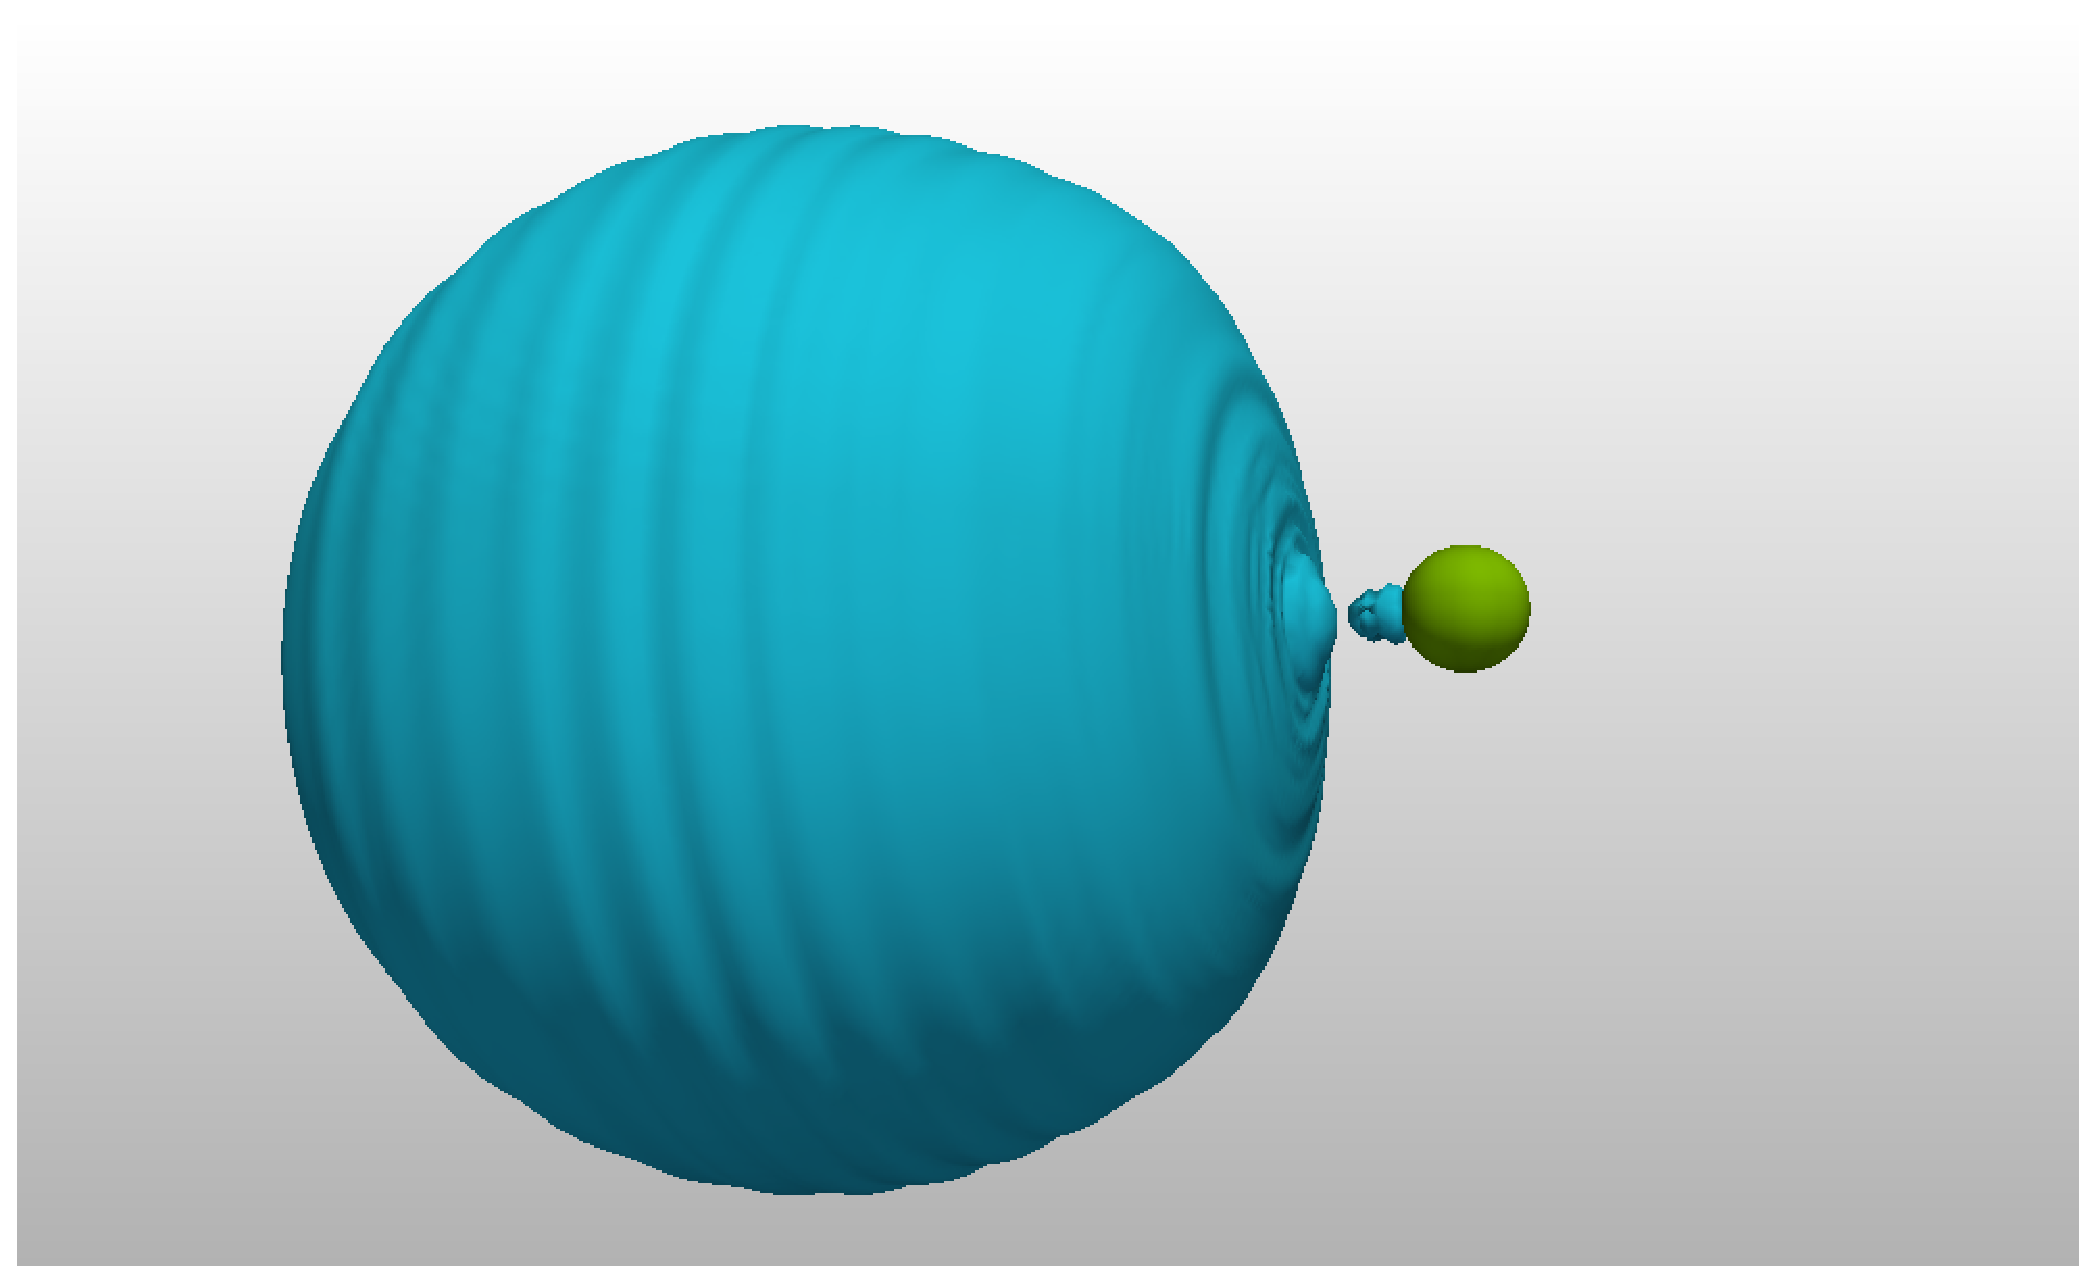
\includegraphics[scale=0.234]{4P-p12-d-snap-linear}}
		\subcaption{Linear exciplex at $t=7.5$ ps \label{fig:4p-p12-d-snap-a}}
	\end{minipage}
\hfill
	\begin{minipage}[c]{0.48\linewidth}
		\fbox{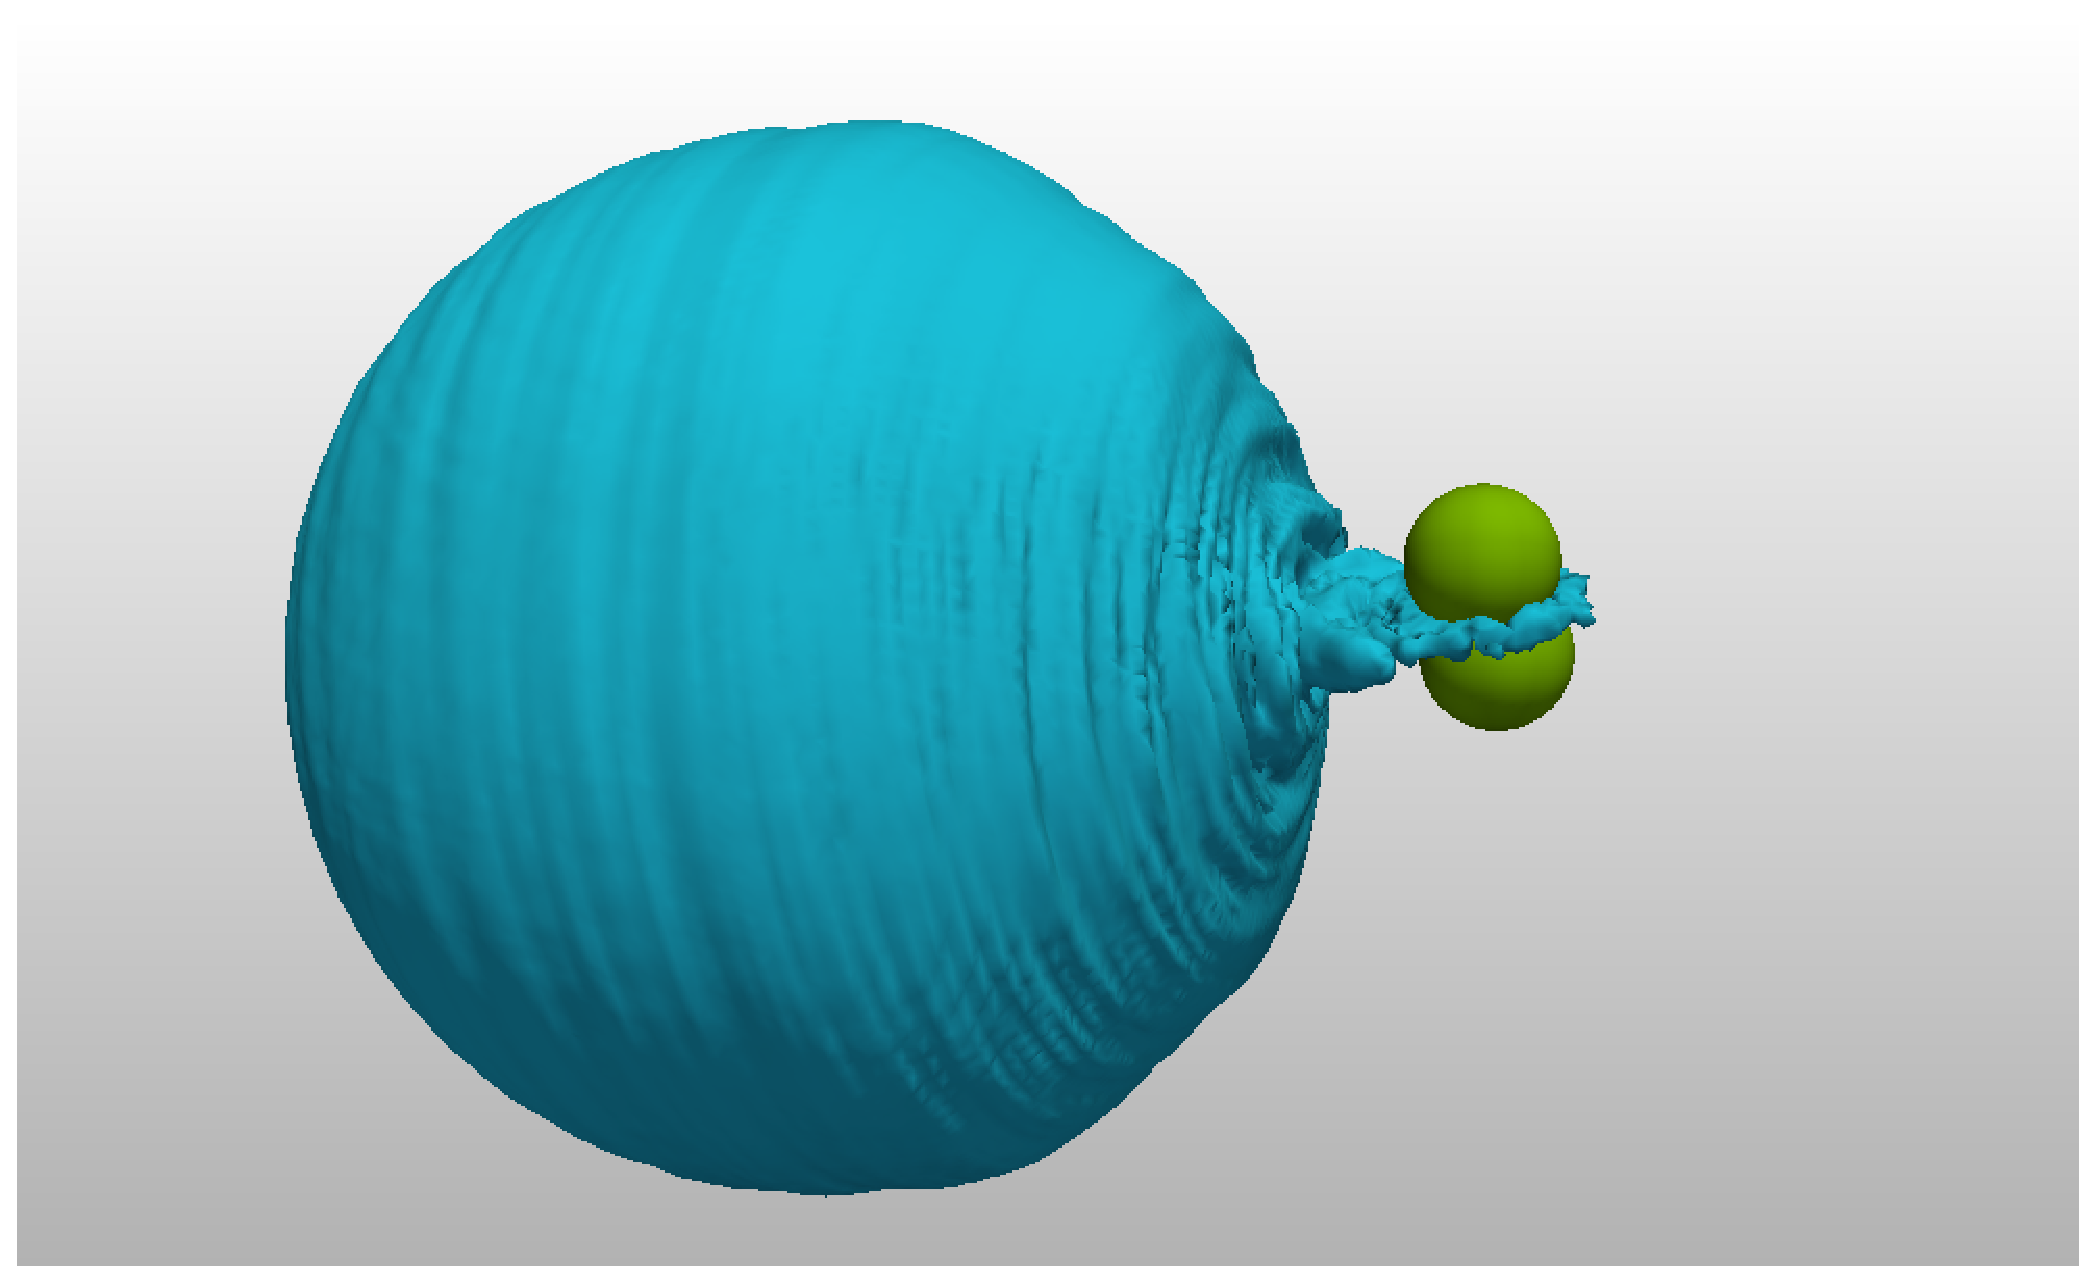
\includegraphics[scale=0.234]{4P-p12-d-snap-ring}}
		\subcaption{Ring exciplex at $t=19.5$ ps \label{fig:4p-p12-d-snap-b}}
	\end{minipage}
\vspace{-0.2\baselineskip}
\label{4P:p12-snap}
\caption{Snapshot of He$_N$ density and bound K exciplex before and after the symmetry breaking, K $p_y$ orbital is schematically represented in the second case to help the interpretation}
\end{figure}

\subsubsection{Investigations on symmetry breaking} 
\indent 
In order to test the hypothesis of the grid effect we worked with a smaller system (90 atoms) an studied the effect of grid size. 
As can be seen in \cittab{table:4P-symb}, the symmetry breaking occurs later and later as we reduce the mesh step size, which corroborates our hypothesis.
\begin{table}[h!]
\centering
\begin{tabular}{|c|c|c|c|c|}
  \hline
  Spatial step size $\delta r$ (\AA) & 0.42 & 0.28 & 0.21 & 0.14 \\
  \hline
  Appearance of the symmetry breaking (ps) & 3.2 & 5.6 & 9.0 & 10.8 \\
  \hline
\end{tabular}
\caption{Evolution of time before the occurrence of symmetry breaking  during a dynamic simulation of  $\Pi_{1/2}$ excitation for different spatial step sizes.}
\label{table:4P-symb}
\end{table}

Now we can understand what is happening: the exciplex formation creates a high density volume which is poorly described by our cubic mesh. This induces asymmetry in the density profile at the surface of the droplet near to K, which induces back an asymmetric interaction and  ends up in the projection of the internal state into an energetically more favorable configuration. 
This also explains why this projection occurs along a well defined axis of our simulation.
%
\subsection{$\Pi_{3/2}$ exciplex formation: beyond symmetry breaking investigations}

\subsubsection{Exciplex formation and symmetry breaking}

Exciting the $\Pi_{3/2}$ state leads without surprise to a linear exciplex (almost identical to \citfig{fig:4p-p12-d-snap-a}) in 4 ps, because we excite in a potential well (\citfig{fig:DIM-4p-pot}). However, in the exact same way as in the $\Pi_{1/2}$ we see that a symmetry breaking occurs. Looking at internal state projections (\citfig{fig:4P-p32-f-proj}) we see that before this symmetry breaking the internal state is actually pure in our basis, as it should, since the $\Omega=3/2$ state is  $\ket{\lambda}=\ket{p_1,+}$ (no other orbital can give $\Omega=3/2$). \\

Comparing trajectories in the $\Pi_{1/2}$  (\citfig{fig:4P-p12-d-pos}) and in the $\Pi_{3/2}$ (\citfig{fig:4P-p32-free-pos}) states shows a difference: in the $\Pi_{3/2}$ state  symmetry breaking occurs during an attempt to leave the droplet while in the $\Pi_{1/2}$ state it happens in a stationary position.

\begin{figure}[h!]
	\centering
	\begin{minipage}[c]{0.48\linewidth}
		% GNUPLOT: LaTeX picture with Postscript
\begingroup
  \makeatletter
  \providecommand\color[2][]{%
    \GenericError{(gnuplot) \space\space\space\@spaces}{%
      Package color not loaded in conjunction with
      terminal option `colourtext'%
    }{See the gnuplot documentation for explanation.%
    }{Either use 'blacktext' in gnuplot or load the package
      color.sty in LaTeX.}%
    \renewcommand\color[2][]{}%
  }%
  \providecommand\includegraphics[2][]{%
    \GenericError{(gnuplot) \space\space\space\@spaces}{%
      Package graphicx or graphics not loaded%
    }{See the gnuplot documentation for explanation.%
    }{The gnuplot epslatex terminal needs graphicx.sty or graphics.sty.}%
    \renewcommand\includegraphics[2][]{}%
  }%
  \providecommand\rotatebox[2]{#2}%
  \@ifundefined{ifGPcolor}{%
    \newif\ifGPcolor
    \GPcolortrue
  }{}%
  \@ifundefined{ifGPblacktext}{%
    \newif\ifGPblacktext
    \GPblacktextfalse
  }{}%
  % define a \g@addto@macro without @ in the name:
  \let\gplgaddtomacro\g@addto@macro
  % define empty templates for all commands taking text:
  \gdef\gplbacktext{}%
  \gdef\gplfronttext{}%
  \makeatother
  \ifGPblacktext
    % no textcolor at all
    \def\colorrgb#1{}%
    \def\colorgray#1{}%
  \else
    % gray or color?
    \ifGPcolor
      \def\colorrgb#1{\color[rgb]{#1}}%
      \def\colorgray#1{\color[gray]{#1}}%
      \expandafter\def\csname LTw\endcsname{\color{white}}%
      \expandafter\def\csname LTb\endcsname{\color{black}}%
      \expandafter\def\csname LTa\endcsname{\color{black}}%
      \expandafter\def\csname LT0\endcsname{\color[rgb]{1,0,0}}%
      \expandafter\def\csname LT1\endcsname{\color[rgb]{0,1,0}}%
      \expandafter\def\csname LT2\endcsname{\color[rgb]{0,0,1}}%
      \expandafter\def\csname LT3\endcsname{\color[rgb]{1,0,1}}%
      \expandafter\def\csname LT4\endcsname{\color[rgb]{0,1,1}}%
      \expandafter\def\csname LT5\endcsname{\color[rgb]{1,1,0}}%
      \expandafter\def\csname LT6\endcsname{\color[rgb]{0,0,0}}%
      \expandafter\def\csname LT7\endcsname{\color[rgb]{1,0.3,0}}%
      \expandafter\def\csname LT8\endcsname{\color[rgb]{0.5,0.5,0.5}}%
    \else
      % gray
      \def\colorrgb#1{\color{black}}%
      \def\colorgray#1{\color[gray]{#1}}%
      \expandafter\def\csname LTw\endcsname{\color{white}}%
      \expandafter\def\csname LTb\endcsname{\color{black}}%
      \expandafter\def\csname LTa\endcsname{\color{black}}%
      \expandafter\def\csname LT0\endcsname{\color{black}}%
      \expandafter\def\csname LT1\endcsname{\color{black}}%
      \expandafter\def\csname LT2\endcsname{\color{black}}%
      \expandafter\def\csname LT3\endcsname{\color{black}}%
      \expandafter\def\csname LT4\endcsname{\color{black}}%
      \expandafter\def\csname LT5\endcsname{\color{black}}%
      \expandafter\def\csname LT6\endcsname{\color{black}}%
      \expandafter\def\csname LT7\endcsname{\color{black}}%
      \expandafter\def\csname LT8\endcsname{\color{black}}%
    \fi
  \fi
    \setlength{\unitlength}{0.0500bp}%
    \ifx\gptboxheight\undefined%
      \newlength{\gptboxheight}%
      \newlength{\gptboxwidth}%
      \newsavebox{\gptboxtext}%
    \fi%
    \setlength{\fboxrule}{0.5pt}%
    \setlength{\fboxsep}{1pt}%
\begin{picture}(4752.00,2880.00)%
    \gplgaddtomacro\gplbacktext{%
      \csname LTb\endcsname%
      \put(708,432){\makebox(0,0)[r]{\strut{}$0$}}%
      \csname LTb\endcsname%
      \put(708,921){\makebox(0,0)[r]{\strut{}$0.2$}}%
      \csname LTb\endcsname%
      \put(708,1411){\makebox(0,0)[r]{\strut{}$0.4$}}%
      \csname LTb\endcsname%
      \put(708,1900){\makebox(0,0)[r]{\strut{}$0.6$}}%
      \csname LTb\endcsname%
      \put(708,2390){\makebox(0,0)[r]{\strut{}$0.8$}}%
      \csname LTb\endcsname%
      \put(708,2879){\makebox(0,0)[r]{\strut{}$1$}}%
      \csname LTb\endcsname%
      \put(840,212){\makebox(0,0){\strut{}$0$}}%
      \csname LTb\endcsname%
      \put(1452,212){\makebox(0,0){\strut{}$2$}}%
      \csname LTb\endcsname%
      \put(2064,212){\makebox(0,0){\strut{}$4$}}%
      \csname LTb\endcsname%
      \put(2677,212){\makebox(0,0){\strut{}$6$}}%
      \csname LTb\endcsname%
      \put(3289,212){\makebox(0,0){\strut{}$8$}}%
      \csname LTb\endcsname%
      \put(3901,212){\makebox(0,0){\strut{}$10$}}%
      \csname LTb\endcsname%
      \put(4513,212){\makebox(0,0){\strut{}$12$}}%
    }%
    \gplgaddtomacro\gplfronttext{%
      \csname LTb\endcsname%
      \put(176,1655){\rotatebox{-270}{\makebox(0,0){\strut{}Intensity (arb. unit)}}}%
      \put(2676,-74){\makebox(0,0){\strut{}Energy (cm$^{-1}$)}}%
      \csname LTb\endcsname%
      \put(1975,1986){\makebox(0,0)[r]{\strut{}$\langle p_{+1},+|$}}%
      \csname LTb\endcsname%
      \put(1975,1766){\makebox(0,0)[r]{\strut{}$\langle p_{-1},+|$}}%
      \csname LTb\endcsname%
      \put(1975,1546){\makebox(0,0)[r]{\strut{}$\langle p_{x},+|$}}%
      \csname LTb\endcsname%
      \put(1975,1326){\makebox(0,0)[r]{\strut{}$\langle p_{y},+|$}}%
    }%
    \gplbacktext
    \put(0,0){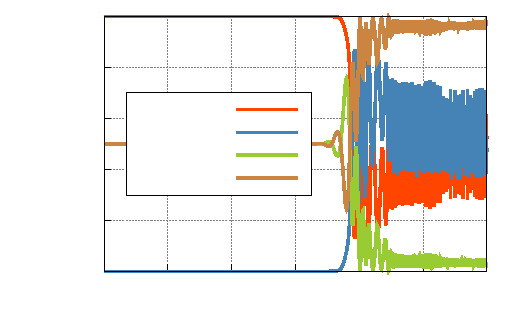
\includegraphics{4P-p32-f-proj}}%
    \gplfronttext
  \end{picture}%
\endgroup

		\vspace{0.2\baselineskip}
		\caption{Evolution of the electronic state as a function of time\label{fig:4P-p32-f-proj}}
	\end{minipage}
\hfill
	\begin{minipage}[c]{0.48\linewidth}
		% GNUPLOT: LaTeX picture with Postscript
\begingroup
  \makeatletter
  \providecommand\color[2][]{%
    \GenericError{(gnuplot) \space\space\space\@spaces}{%
      Package color not loaded in conjunction with
      terminal option `colourtext'%
    }{See the gnuplot documentation for explanation.%
    }{Either use 'blacktext' in gnuplot or load the package
      color.sty in LaTeX.}%
    \renewcommand\color[2][]{}%
  }%
  \providecommand\includegraphics[2][]{%
    \GenericError{(gnuplot) \space\space\space\@spaces}{%
      Package graphicx or graphics not loaded%
    }{See the gnuplot documentation for explanation.%
    }{The gnuplot epslatex terminal needs graphicx.sty or graphics.sty.}%
    \renewcommand\includegraphics[2][]{}%
  }%
  \providecommand\rotatebox[2]{#2}%
  \@ifundefined{ifGPcolor}{%
    \newif\ifGPcolor
    \GPcolortrue
  }{}%
  \@ifundefined{ifGPblacktext}{%
    \newif\ifGPblacktext
    \GPblacktextfalse
  }{}%
  % define a \g@addto@macro without @ in the name:
  \let\gplgaddtomacro\g@addto@macro
  % define empty templates for all commands taking text:
  \gdef\gplbacktext{}%
  \gdef\gplfronttext{}%
  \makeatother
  \ifGPblacktext
    % no textcolor at all
    \def\colorrgb#1{}%
    \def\colorgray#1{}%
  \else
    % gray or color?
    \ifGPcolor
      \def\colorrgb#1{\color[rgb]{#1}}%
      \def\colorgray#1{\color[gray]{#1}}%
      \expandafter\def\csname LTw\endcsname{\color{white}}%
      \expandafter\def\csname LTb\endcsname{\color{black}}%
      \expandafter\def\csname LTa\endcsname{\color{black}}%
      \expandafter\def\csname LT0\endcsname{\color[rgb]{1,0,0}}%
      \expandafter\def\csname LT1\endcsname{\color[rgb]{0,1,0}}%
      \expandafter\def\csname LT2\endcsname{\color[rgb]{0,0,1}}%
      \expandafter\def\csname LT3\endcsname{\color[rgb]{1,0,1}}%
      \expandafter\def\csname LT4\endcsname{\color[rgb]{0,1,1}}%
      \expandafter\def\csname LT5\endcsname{\color[rgb]{1,1,0}}%
      \expandafter\def\csname LT6\endcsname{\color[rgb]{0,0,0}}%
      \expandafter\def\csname LT7\endcsname{\color[rgb]{1,0.3,0}}%
      \expandafter\def\csname LT8\endcsname{\color[rgb]{0.5,0.5,0.5}}%
    \else
      % gray
      \def\colorrgb#1{\color{black}}%
      \def\colorgray#1{\color[gray]{#1}}%
      \expandafter\def\csname LTw\endcsname{\color{white}}%
      \expandafter\def\csname LTb\endcsname{\color{black}}%
      \expandafter\def\csname LTa\endcsname{\color{black}}%
      \expandafter\def\csname LT0\endcsname{\color{black}}%
      \expandafter\def\csname LT1\endcsname{\color{black}}%
      \expandafter\def\csname LT2\endcsname{\color{black}}%
      \expandafter\def\csname LT3\endcsname{\color{black}}%
      \expandafter\def\csname LT4\endcsname{\color{black}}%
      \expandafter\def\csname LT5\endcsname{\color{black}}%
      \expandafter\def\csname LT6\endcsname{\color{black}}%
      \expandafter\def\csname LT7\endcsname{\color{black}}%
      \expandafter\def\csname LT8\endcsname{\color{black}}%
    \fi
  \fi
    \setlength{\unitlength}{0.0500bp}%
    \ifx\gptboxheight\undefined%
      \newlength{\gptboxheight}%
      \newlength{\gptboxwidth}%
      \newsavebox{\gptboxtext}%
    \fi%
    \setlength{\fboxrule}{0.5pt}%
    \setlength{\fboxsep}{1pt}%
\begin{picture}(4752.00,2880.00)%
    \gplgaddtomacro\gplbacktext{%
      \csname LTb\endcsname%
      \put(682,432){\makebox(0,0)[r]{\strut{}$26$}}%
      \csname LTb\endcsname%
      \put(682,921){\makebox(0,0)[r]{\strut{}$27$}}%
      \csname LTb\endcsname%
      \put(682,1411){\makebox(0,0)[r]{\strut{}$28$}}%
      \csname LTb\endcsname%
      \put(682,1900){\makebox(0,0)[r]{\strut{}$29$}}%
      \csname LTb\endcsname%
      \put(682,2390){\makebox(0,0)[r]{\strut{}$30$}}%
      \csname LTb\endcsname%
      \put(682,2879){\makebox(0,0)[r]{\strut{}$31$}}%
      \csname LTb\endcsname%
      \put(814,212){\makebox(0,0){\strut{}$0$}}%
      \csname LTb\endcsname%
      \put(1554,212){\makebox(0,0){\strut{}$5$}}%
      \csname LTb\endcsname%
      \put(2294,212){\makebox(0,0){\strut{}$10$}}%
      \csname LTb\endcsname%
      \put(3033,212){\makebox(0,0){\strut{}$15$}}%
      \csname LTb\endcsname%
      \put(3773,212){\makebox(0,0){\strut{}$20$}}%
      \csname LTb\endcsname%
      \put(4513,212){\makebox(0,0){\strut{}$25$}}%
    }%
    \gplgaddtomacro\gplfronttext{%
      \csname LTb\endcsname%
      \put(176,1655){\rotatebox{-270}{\makebox(0,0){\strut{}K relative position (\AA)}}}%
      \put(2663,-74){\makebox(0,0){\strut{}Time (ps)}}%
    }%
    \gplbacktext
    \put(0,0){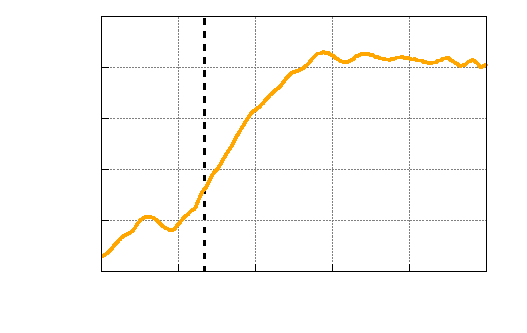
\includegraphics{4P-p32-free-pos}}%
    \gplfronttext
  \end{picture}%
\endgroup

		\vspace{0.2\baselineskip}
		\caption{Distance between K and He$_N$ centers of mass as a function of time\label{fig:4P-p32-free-pos}}
	\end{minipage}
\end{figure}

\subsubsection{Fixing internal state evolution}

We can use the fact that there is no possible evolution for the internal state\footnote{At least in our cylindrical framework} to fix it instead of let it freely evolve. 
As can be seen in \citfig{fig:4P-p32-fx-snap}, in that case the linear exciplex leaves the droplet after the symmetry breaking (\citfig{fig:4P-p32-fx-snap}).

\begin{figure}[h!]
\centering
	\begin{minipage}[c]{0.48\linewidth}
		\fbox{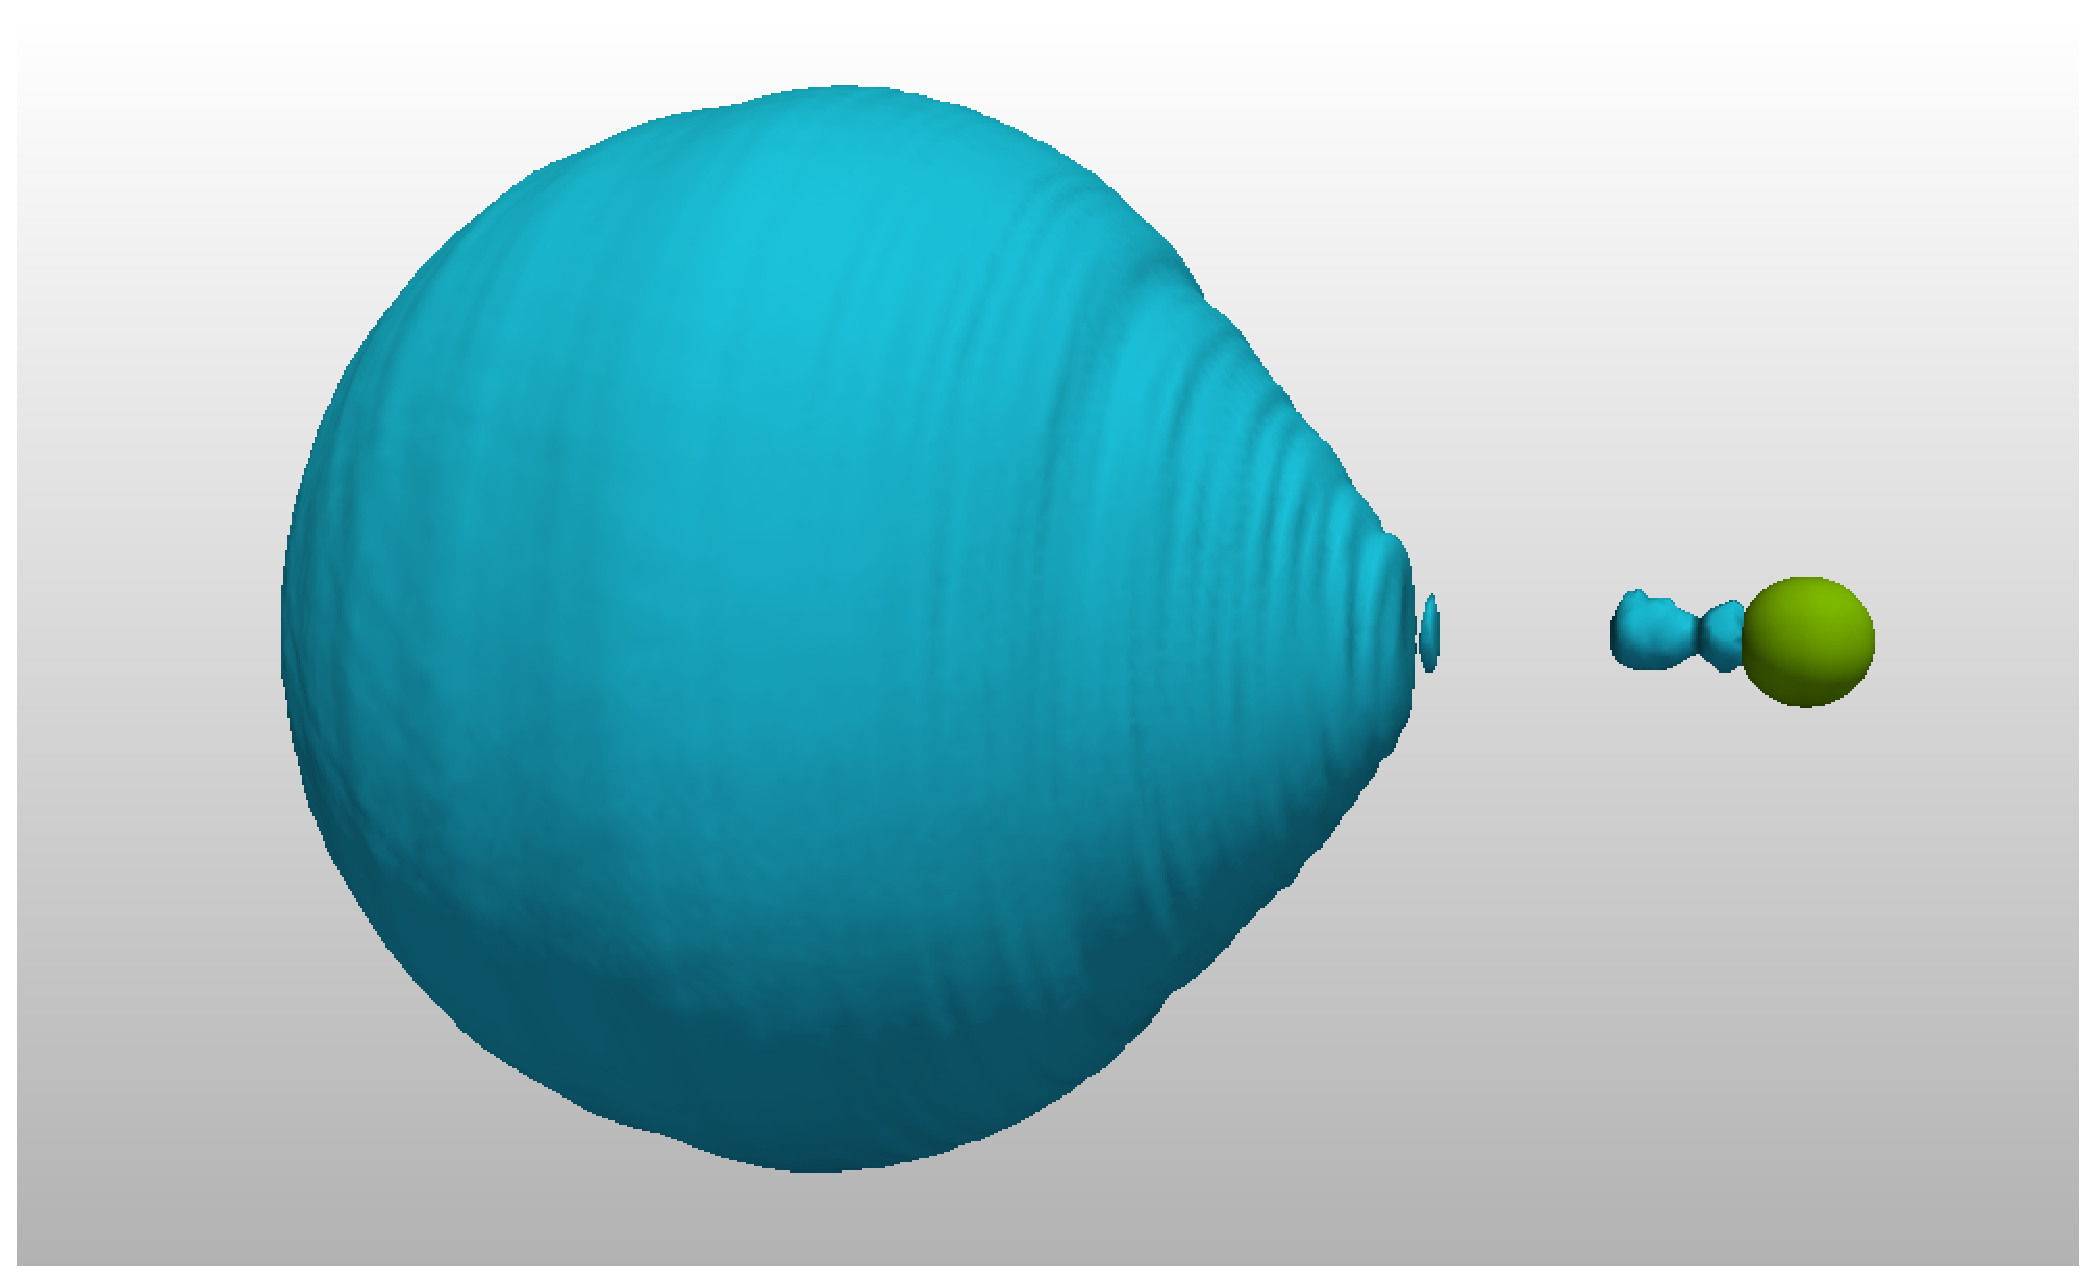
\includegraphics[scale=0.234]{4P-p32-fx-snap}}
		\caption{Snapshot of He$_N$ density with a linear KHe$_n$ exciplex leaving the droplet at $t=18.5$ ps\label{fig:4P-p32-fx-snap}}
	\end{minipage}
\hfill
	\begin{minipage}[c]{0.48\linewidth}
		% GNUPLOT: LaTeX picture with Postscript
\begingroup
  \makeatletter
  \providecommand\color[2][]{%
    \GenericError{(gnuplot) \space\space\space\@spaces}{%
      Package color not loaded in conjunction with
      terminal option `colourtext'%
    }{See the gnuplot documentation for explanation.%
    }{Either use 'blacktext' in gnuplot or load the package
      color.sty in LaTeX.}%
    \renewcommand\color[2][]{}%
  }%
  \providecommand\includegraphics[2][]{%
    \GenericError{(gnuplot) \space\space\space\@spaces}{%
      Package graphicx or graphics not loaded%
    }{See the gnuplot documentation for explanation.%
    }{The gnuplot epslatex terminal needs graphicx.sty or graphics.sty.}%
    \renewcommand\includegraphics[2][]{}%
  }%
  \providecommand\rotatebox[2]{#2}%
  \@ifundefined{ifGPcolor}{%
    \newif\ifGPcolor
    \GPcolortrue
  }{}%
  \@ifundefined{ifGPblacktext}{%
    \newif\ifGPblacktext
    \GPblacktextfalse
  }{}%
  % define a \g@addto@macro without @ in the name:
  \let\gplgaddtomacro\g@addto@macro
  % define empty templates for all commands taking text:
  \gdef\gplbacktext{}%
  \gdef\gplfronttext{}%
  \makeatother
  \ifGPblacktext
    % no textcolor at all
    \def\colorrgb#1{}%
    \def\colorgray#1{}%
  \else
    % gray or color?
    \ifGPcolor
      \def\colorrgb#1{\color[rgb]{#1}}%
      \def\colorgray#1{\color[gray]{#1}}%
      \expandafter\def\csname LTw\endcsname{\color{white}}%
      \expandafter\def\csname LTb\endcsname{\color{black}}%
      \expandafter\def\csname LTa\endcsname{\color{black}}%
      \expandafter\def\csname LT0\endcsname{\color[rgb]{1,0,0}}%
      \expandafter\def\csname LT1\endcsname{\color[rgb]{0,1,0}}%
      \expandafter\def\csname LT2\endcsname{\color[rgb]{0,0,1}}%
      \expandafter\def\csname LT3\endcsname{\color[rgb]{1,0,1}}%
      \expandafter\def\csname LT4\endcsname{\color[rgb]{0,1,1}}%
      \expandafter\def\csname LT5\endcsname{\color[rgb]{1,1,0}}%
      \expandafter\def\csname LT6\endcsname{\color[rgb]{0,0,0}}%
      \expandafter\def\csname LT7\endcsname{\color[rgb]{1,0.3,0}}%
      \expandafter\def\csname LT8\endcsname{\color[rgb]{0.5,0.5,0.5}}%
    \else
      % gray
      \def\colorrgb#1{\color{black}}%
      \def\colorgray#1{\color[gray]{#1}}%
      \expandafter\def\csname LTw\endcsname{\color{white}}%
      \expandafter\def\csname LTb\endcsname{\color{black}}%
      \expandafter\def\csname LTa\endcsname{\color{black}}%
      \expandafter\def\csname LT0\endcsname{\color{black}}%
      \expandafter\def\csname LT1\endcsname{\color{black}}%
      \expandafter\def\csname LT2\endcsname{\color{black}}%
      \expandafter\def\csname LT3\endcsname{\color{black}}%
      \expandafter\def\csname LT4\endcsname{\color{black}}%
      \expandafter\def\csname LT5\endcsname{\color{black}}%
      \expandafter\def\csname LT6\endcsname{\color{black}}%
      \expandafter\def\csname LT7\endcsname{\color{black}}%
      \expandafter\def\csname LT8\endcsname{\color{black}}%
    \fi
  \fi
    \setlength{\unitlength}{0.0500bp}%
    \ifx\gptboxheight\undefined%
      \newlength{\gptboxheight}%
      \newlength{\gptboxwidth}%
      \newsavebox{\gptboxtext}%
    \fi%
    \setlength{\fboxrule}{0.5pt}%
    \setlength{\fboxsep}{1pt}%
\begin{picture}(4752.00,2880.00)%
    \gplgaddtomacro\gplbacktext{%
      \csname LTb\endcsname%
      \put(682,432){\makebox(0,0)[r]{\strut{}$26$}}%
      \csname LTb\endcsname%
      \put(682,921){\makebox(0,0)[r]{\strut{}$27$}}%
      \csname LTb\endcsname%
      \put(682,1411){\makebox(0,0)[r]{\strut{}$28$}}%
      \csname LTb\endcsname%
      \put(682,1900){\makebox(0,0)[r]{\strut{}$29$}}%
      \csname LTb\endcsname%
      \put(682,2390){\makebox(0,0)[r]{\strut{}$30$}}%
      \csname LTb\endcsname%
      \put(682,2879){\makebox(0,0)[r]{\strut{}$31$}}%
      \csname LTb\endcsname%
      \put(814,212){\makebox(0,0){\strut{}$0$}}%
      \csname LTb\endcsname%
      \put(1554,212){\makebox(0,0){\strut{}$5$}}%
      \csname LTb\endcsname%
      \put(2294,212){\makebox(0,0){\strut{}$10$}}%
      \csname LTb\endcsname%
      \put(3033,212){\makebox(0,0){\strut{}$15$}}%
      \csname LTb\endcsname%
      \put(3773,212){\makebox(0,0){\strut{}$20$}}%
      \csname LTb\endcsname%
      \put(4513,212){\makebox(0,0){\strut{}$25$}}%
    }%
    \gplgaddtomacro\gplfronttext{%
      \csname LTb\endcsname%
      \put(176,1655){\rotatebox{-270}{\makebox(0,0){\strut{}K relative position (\AA)}}}%
      \put(2663,-74){\makebox(0,0){\strut{}Time (ps)}}%
      \csname LTb\endcsname%
      \put(3526,1765){\makebox(0,0)[r]{\strut{}Free}}%
      \csname LTb\endcsname%
      \put(3526,1545){\makebox(0,0)[r]{\strut{}Fixed}}%
    }%
    \gplbacktext
    \put(0,0){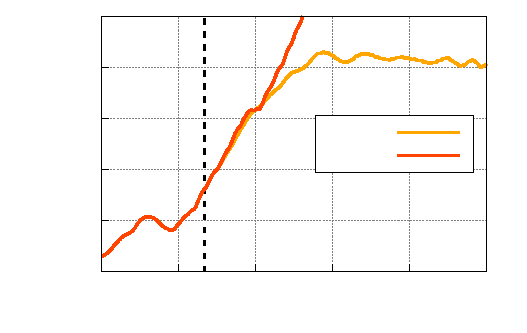
\includegraphics{4P-p32-fxd-pos}}%
    \gplfronttext
  \end{picture}%
\endgroup

		\vspace{0.2\baselineskip}
		\caption{Distance between K and He$_N$ centers of mass as a function of time, for fixed and free $\ket{\lambda}$\label{fig:4P-p32-fxd-pos}}
	\end{minipage}
\end{figure}

Comparing trajectories in the case of a free or fixed electronic state evolution (\citfig{fig:4P-p32-fxd-pos}) shows that the leaving exciplex seems to be the natural response of this system. 
Nevertheless when we let the internal state evolve, the system finds a way to handle a new symmetry which is the formation of a ring exciplex that is more cubic symmetry friendly.\\

We might be tempted to interpret these symmetry breakings as a possibility that could occur in a real experiment, due to spatial distortion of the droplet or any external perturbation. 
Hints for ring exciplex stability in the Cs case have been found \cite{Zbi2005}.
But this clearly remains an open question for potassium that requires further investigations.

\subsection{Comparison with exprimental data}

Alkali doped droplets have been studied extensively \cite{Sti1996,Lac2011,Lac2012,Bru2001,Her2012,Log2014,Log2015,Van2017}. 
Nevertheless there are only two articles that investigated the dynamics following $4p\leftarrow 4s$ excitation of a K-doped droplet: \cite{Reh2000A,Reh2000B} (single article split in two) and \cite{Sch2001}. 
\cite{Reh2000A,Reh2000B} collected dispersed emission spectra using reversed time-correlated single photon counting while \cite{Sch2001} used femtosecond pumb-probe spectroscopy. 
Both report the formation of exciplexes in the $\Pi$ states and desorption in the $\Sigma$ state. 
Both show that the most abundant product species is KHe.
They also report a $\sim$10\% KHe$_2$ production. \cite{Sch2001} even shows that KHe$_n$ exciplexes are formed with $n=3,4$ (2.3\% both) and $n=5$ (0.5\%). 
Nevertheless there is a huge discrepancy in the measured formation time scale. 
\cite{Reh2000A,Reh2000B} gives 50 $\pm$ 20 ps ($\Pi_{3/2}$) and 7.9 ns ($\Pi_{1/2}$),  whereas \cite{Sch2001} cannot resolve the two $\Pi$ states but gives 180 $\pm$ 60 fs (KHe) and 204$ \pm$ 60 fs (KHe$_2$).\\ 

After discussions with the authors of \cite{Sch2001} during a conference\footnote{Quantum Fluid Clusters conference, Obergurgl (Austria), June 7-9, 2017, where I presented a poster on my results}, it appears that their results on the time scale could be wrong due to a too high repetition rate of the exciting laser. 
They could have been exciting the $5p$ state (24701.382 cm$^{-1}$ and 24720.139 cm$^{-1}$ \cite{Nist}) trough a two-photon process. \\

We have seen that our simulation describes well the formation of exciplexes.
In particular the linear exciplex shape is consistent with the  K-He observed experimentally\footnote{He-TDDFT has been found to give non-integer numbers of atom in exciplexes, so we may only use qualitative arguments based on 3D representation} but no evidence for linear He-K-He (KHe$_2$) was found. The small proportion of higher $n$ exciplexes observed experimentally could be a hint for the existence of ring shaped configurations.\\

Concerning the time scale in our simulations, in $\Pi_{3/2}$ excitation the potassium trajectory shows that the exciplex starts to leave within 5 ps, the symmetry breaking occurs after the beginning of desorption. 
Fixing the electronic state demonstrates that this desorption is the physical answer of the system rather than bound configuration. 
In the $\Pi_{1/2}$ state we observe a bouncing free potassium (the simulation is still running but the time scale to reach a stationary state may be $\sim$ ns).
We could imagine that once in an equilibrium position, some tunneling effect may occur through the tiny barrier leading to exciplex formation within a few ns, see model presented in \cite{Reh2000A,Reh2000B}.
Finally, in the displaced $\Pi_{1/2}$ we cannot fix the internal state but during the formation of the linear exciplex the internal state goes to $\ket{p_1}$, which is the same than in $\Pi_{3/2}$.
This is why we can expect a departing exciplex (and not bound) within 15 ps.\\

These results are closer to the ones from \cite{Reh2000A,Reh2000B} which give 50 ps ($\Pi_{3/2}$) and 7.9 ns ($\Pi_{1/2}$) than \cite{Sch2001} which give 180 fs for both. 
This is probably explained by the setup dysfunctional described earlier.
The only true discrepancy that remains with \cite{Reh2000A,Reh2000B} is the $\Pi_{1/2}$ displaced excitation. We do not get a clear explanation, however as it is a turning point this could be a rare case in experiments. 
This could also be a limitation of our simulations.